\documentclass[11pt,a4paper,twoside]{article}
\usepackage[utf8]{inputenc}

%\usepackage{fancyhdr}
%\pagestyle{fancy}
% ***************************************************************************************************************************************
% math and graphics 
\usepackage{amsmath,amsfonts,amssymb,amsthm}
\usepackage{thmtools}
\usepackage{mathtools}
\usepackage{braket}
\usepackage{graphicx,svg,subcaption}
\usepackage{tikz}
\usepackage{tikz-3dplot}
\usepackage{pgfplots}
\usepackage{listings}
\usepackage{sagetex}
\usepackage{pdfpages}
\usepackage{todonotes}
\usepackage{braids}


% ***************************************************************************************************************************************
% TikZ libraries
\usetikzlibrary{arrows, calc,decorations.markings,cd,external}
\tikzexternalize[prefix=figures/, figure name=figure_subsection\thesubsection_no]
%\input{./tikzcd_hack.tex}
\usepackage{etoolbox}
\AtBeginEnvironment{tikzcd}{\tikzexternaldisable}
\AtEndEnvironment{tikzcd}{\tikzexternalenable}
\newcommand{\ruggedtodo}[2][]{\tikzexternaldisable\todo[#1]{#2}\tikzexternalenable}
\makeatletter 
\tikzstyle{inlinenotestyle} = [
    draw=\@todonotes@currentbordercolor,
    fill=\@todonotes@currentbackgroundcolor,
    line width=0.5pt,
    inner sep = 0.8 ex,
    rounded corners=4pt]

\renewcommand{\@todonotes@drawInlineNote}{%
        {
\begin{tikzpicture}[remember picture,baseline=(current bounding box.base)]%
            \draw node[inlinenotestyle,font=\@todonotes@sizecommand, anchor=base,baseline]{%
              \if@todonotes@authorgiven%
                {\noindent \@todonotes@sizecommand \@todonotes@author:\,\@todonotes@text}%
              \else%
                {\noindent \@todonotes@sizecommand \@todonotes@text}%
              \fi};%
           \end{tikzpicture}}}%
\makeatother   
%\AtBeginEnvironment{tikzpicture}{\renewcommand{\thisName}{\the\value{chapter}\relax chapter}\tikzsetnextfilename{\thisName}}
%\newcommand{\thisName}{}

% ***************************************************************************************************************************************
% appearance
%\newcommand{\changefont}{%
%    \fontsize{9}{11}\selectfont
%}
%\fancyhf{}
%\fancyhead[LE, RO]{\thepage}
%\fancyhead[LO]{\changefont \sffamily \nouppercase{\rightmark}} %section
%\fancyhead[RE]{\changefont \sffamily \nouppercase{\leftmark}} %chapter

\newcommand{\figref}[1]{\textsf{Figure \ref{#1}}}
\renewcommand{\eqref}[1]{\textsf{Equation (\ref{#1})}}


\usepackage[colorlinks=true]{hyperref}
%\usepackage[hidelinks=true]{hyperref}
%\usepackage[left=2.5cm,right=2.5cm,top=2cm,bottom=2cm,includehead]{geometry}
%\usepackage[left=3.5cm,right=3.5cm,top=2.5cm,bottom=4cm,includehead]{geometry}
%\usepackage[left=3.5cm,right=3.5cm,top=3cm,bottom=5cm]{geometry}
\usepackage[inner=3.3cm,textwidth=400pt, top=3.2cm,bottom=4.8cm, includehead]{geometry}
\usepackage{ragged2e}
\usepackage{microtype}
\usepackage{hhline}
\usepackage{caption}
\usepackage{color}
\usepackage{amsfonts}

%\addtokomafont{pageheadfoot}{\scshape\small}
\renewcommand{\theequation}{{\textsf{\thechapter.\arabic{equation}}}}

\definecolor{mygray}{rgb}{0.5,0.5,0.5}
%\definecolor{myblue}{rgb}{0,0,1}
%\definecolor{mymauve}{rgb}{0.58,0,0.82}
\definecolor{myblue}{rgb}{0,0,0}
\definecolor{mymauve}{rgb}{0,0,0}

\lstset{ %
  backgroundcolor=\color{white},   % choose the background color; you must add \usepackage{color} or \usepackage{xcolor}; should come as last argument
  basicstyle=\footnotesize\ttfamily,        % the size of the fonts that are used for the code
  breakatwhitespace=false,         % sets if automatic breaks should only happen at whitespace
  breaklines=true,                 % sets automatic line breaking
  captionpos=b,                    % sets the caption-position to bottom
  commentstyle=\color{mygray},    % comment style
  deletekeywords={...},            % if you want to delete keywords from the given language
  escapeinside={\%*}{*)},          % if you want to add LaTeX within your code
  extendedchars=true,              % lets you use non-ASCII characters; for 8-bits encodings only, does not work with UTF-8
  frame=single,	                   % adds a frame around the code
  keepspaces=true,                 % keeps spaces in text, useful for keeping indentation of code (possibly needs columns=flexible)
  keywordstyle=\color{myblue},       % keyword style
  language=Python,                 % the language of the code
  morekeywords={*,...},            % if you want to add more keywords to the set
  numbers=left,                    % where to put the line-numbers; possible values are (none, left, right)
  numbersep=5pt,                   % how far the line-numbers are from the code
  numberstyle=\tiny, % the style that is used for the line-numbers
  rulecolor=\color{black},         % if not set, the frame-color may be changed on line-breaks within not-black text (e.g. comments (green here))
  showspaces=false,                % show spaces everywhere adding particular underscores; it overrides 'showstringspaces'
  showstringspaces=false,          % underline spaces within strings only
  showtabs=false,                  % show tabs within strings adding particular underscores
  stepnumber=5,                    % the step between two line-numbers. If it's 1, each line will be numbered
  stringstyle=\color{mymauve},     % string literal style
  tabsize=2,	                   % sets default tabsize to 2 spaces
  %title=                   % show the filename of files included with \lstinputlisting; also try caption instead of title
}


% ***************************************************************************************************************************************
% additional behavior: index, bib
\usepackage{imakeidx,url}
\usepackage[labelfont=sf]{caption}
\usepackage[nottoc]{tocbibind}
\usepackage[titletoc,header]{appendix}
\usepackage{epigraph}
%\setcounter{secnumdepth}{1}
%\usepackage{refstyle}
\makeindex[intoc]
\allowdisplaybreaks 


% ***************************************************************************************************************************************
% environments
\newcounter{conj}
\renewcommand{\theconj}{\Alph{conj}}
\newcounter{factoid}

\declaretheorem[style=definition,qed=$\triangle$,numberwithin=section,postheadhook={~\\ \indent}]{definition}
\declaretheorem[style=remark,qed=$\blacktriangle$,sibling=definition,postheadhook={~\\ \indent}]{remark}
\declaretheorem[style=plain,sibling=definition]{theorem}
\declaretheorem[style=plain,numberlike=conj,qed=$\blacktriangle$]{conjecture}
\declaretheorem[style=plain,sibling=definition]{lemma}
\declaretheorem[style=definition,numberlike=factoid]{fact}
\declaretheorem[style=plain,sibling=definition]{proposition}
\declaretheorem[style=plain,sibling=definition]{example}
% ***********************************************************   commands  ***********************************************************
% ********************** MATH ******************************
\renewcommand{\phi}{\varphi}
\renewcommand{\theta}{\vartheta}
\newcommand{\hilbert}[1]{\mathcal{H}_{#1}}
\newcommand{\tensor}{\otimes}
\newcommand{\inv}{^{-1}}
\newcommand{\eqasd}{•}
\newcommand{\interior}[1]{#1^\circ}
\newcommand{\markedPoint}{\star}
\newcommand{\rotatedmultiplication}[1]{\stackrel{#1}{\curvearrowleft}\,}
\newcommand\at[2]{\left.#1\right|_{#2}}
\newcommand{\morphism}[1]{\xrightarrow{#1}}
\DeclarePairedDelimiter{\floor}{\lfloor}{\rfloor}
\DeclarePairedDelimiter{\ceil}{\lceil}{\rceil}


\renewcommand{\vec}[1]{\mathbf{#1}}

\DeclareMathOperator{\im}{im}
\DeclareMathOperator{\id}{id}
\DeclareMathOperator{\mult}{mult}
\DeclareMathOperator{\rot}{rot}
\DeclareMathOperator{\End}{End}
\DeclareMathOperator{\supp}{supp}
\newcommand{\catname}[1]{{\normalfont\textbf{#1}}}
\renewcommand{\Re}{\operatorname{Re}}
\renewcommand{\Im}{\operatorname{Im}}

% ********************* Other ****************************
\newcommand{\bigno}{\bigskip\noindent}


\author{Johannes Berger, Tobias J Osborne}
\title{On Perfect Planar Tangles}
\date{}

% DOCUMENT
\begin{document}\pagestyle{headings}
\maketitle
%\listoftodos
\begin{center}
	\begin{minipage}{0.8\textwidth}
		\textsc{Abstract.} We propose the concept of \emph{perfect planar tangles}, which can serve as a generalization of biunitaries as well as perfect tensors.
	\end{minipage}
\end{center}


%\chapter*{Introduction}\addcontentsline{toc}{chapter}{Introduction}
%	\setlength{\epigraphwidth}{0.61\textwidth}
%\textit{I have not seen far, despite standing on the shoulders of giants.}
\epigraph{\textit{Rigor cleans the window through which intuition shines.}}{Elliot D.\ Cooper\footnotemark} \footnotetext{\cite{cooper2011mathematical}}

\noindent 
Maldacena's initial discovery \cite{maldacena1999large} of evidence for the AdS/CFT correspondence in 1997 has, without a doubt, greatly shaped the modern physics community.
This remarkable (proposed) duality between theories of quantum gravity in $(d+1+1)$-dimensional anti-de Sitter space and conformal field theories on its $(d+1)$-dimensional conformal boundary has provided a lot of new insights about \emph{quantum gravity} as a whole. 

One facet of this is a manifest connection between entanglement and geometry, resulting in the famous Ryu-Takayanagi conjecture \cite{ryu2006holographic}, which asserts that the entanglement entropy of a a region in the boundary CFT is proportional to the area of a specific surface in the bulk gravitational theory.

There are some problems, for example the boundary dual of a \emph{local} bulk operator, see  \cite{Pastawski2015Holographic} and in particular Figure 9 of \cite{almheiri2015bulk}. However, this problem was resolved in \cite{almheiri2015bulk}, using the theory of quantum error correction to translate local bulk operators to \emph{logical} operators on the boundary. 

Prompted by this, Pastawski, Yoshida, Harlow, and Preskill \cite{Pastawski2015Holographic} proposed a family of exactly solvable toy models for the holographic correspondence, using \emph{holographic states}, i.e.\ tensor networks that are built from so-called \emph{perfect tensors}, which are associated with quantum error correcting codes \cite{raissi2017constructingQECC}. These states, sitting in a space slice of $AdS_{2+1}$, realize some interesting properties: Among other things, they satisfy a discrete version of Ryu-Takayanagi when the boundary region is connected.

In this thesis, we take tensors that are only \emph{planarly} perfect --- not quite perfect but sufficiently so --- and generalize them to the setting of planar algebras (a purely pictorial endeavor, for all intents and purposes) with the aim of finding new constructions and realizations.

\bigskip
In the first chapter we motivate this thesis for a broader audience by showing a natural progression of extracting the notion of \emph{perfect tensor} from an easy quantum-mechanical context. We then define tensor networks, and use the inherent graphical calculus to whet the appetite for what's to come, namely a lot of calculations with pictures. We also briefly mention what perfect tensors have been used for, e.g.\ in the paper \cite{Pastawski2015Holographic} that introduced them.

We hint at the next chapters by defining the most important foundational part of this thesis, namely the \emph{Temperley-Lieb algebras}, first introduced in \cite{temperley1971relations} and turned into a diagrammatic algebra in \cite{kauffman1987state}.

\bigskip
The second chapter is a quick introduction to the theory of \emph{planar algebras}, originally published by Jones in 1999 \cite{jones1999planar1}, a pictorial language for the standard invariant of a subfactor. Interestingly, the question whether there exists a ``functorial'' connection between finite-index subfactors and CFTs is an area of active research. But it is unfortunately not yet known whether every subfactor gives rise to a CFT, or, if that is the case, if the subfactor can then be recovered at all \cite{oberwolfach}.

\bigskip
The heart of this thesis is undoubtedly the third chapter, where we propose the concept of \emph{perfect tangles} --- elements in a planar ${}^*$-algebra that are unitary (up to nonzero scalar), and all of whose rotations are unitary as well. These new mathematical objects can serve as a generalization of a few notions, including \emph{biunitaries} in planar algebras, and (planarly) perfect tensors. While this alone certainly serves as a motivation and justification for studying perfect tangles, another reason is that it's just interesting to see whether these at first glance highly artificial things even exist and what they look like --- and it's a fun \emph{Spielerei}.

But not only are we doing that, we are also discussing how to simplify calculations considerably, at least in the Temperley-Lieb case, followed by a discussion about the support of perfect TL tangles, and the connection to the braid group. 

Then, after stating and proving a suggestion by Jones, namely a construction of large perfect tangles from smaller perfect tangles using braiding-based intuition coming from the Temperley-Lieb case, we conjecture that this is actually valid in a more general setting, and in particular is true when applied to planarly perfect tensors. We then ask the natural question whether a certain well-defined way of constructing large tangles from smaller perfect tangles always yields something perfect, and whether this assignment is injective. This question remains open, despite good evidence and handwaving supporting an affirmative answer.

If all of this is true then we have found a way of taking planarly perfect tensors and constructing tensor networks that are themselves planarly perfect, allowing for a lot of different geometries.

After the theoretical part of the chapter, we can finally present a few examples of perfect tangles that have been found. Many of them are indeed in the Temperley-Lieb planar algebra --- an initial object in the category of subfactor planar algebras --- but a few are also in trivalent categories.

\bigskip
Finally, the appendix consists of 
\begin{itemize}
\item[\textsf{A.}] a brief introduction to category theory, to fix conventions and help clarify the definition of trivalent categories.
\item[\textsf{B.}] a more rigorous formulation of planar tangles following \cite{KODIYALAM:OnPlanarAlgebras}.
\item[\textsf{C.}] some bits and pieces of the code produced for this thesis. The full code can be found here: \url{github.com/zerschmetterling/ppt_code}
\end{itemize}

\section{Planar Algebras}
	\index{Planar Algebras}
	Although we will mostly be working in Temperley-Lieb (TL) algebras, we will introduce the notion of a \emph{planar algebra} in this chapter. One of the reasons for this is that the collection of TL algebras can be equipped with a planar structure, yielding the Temperley-Lieb planar algebra, and that trivalent categories have a deep connection to planar algebras as well. The other reason is that our main definitions and some theorems work in planar algebras in general, that is, independent of the nature of the things we `put into the boxes'.

Planar algebras were first defined by Jones in \cite{jones1999planar1}, to help in the study of subfactors. They are designed to graphically capture multilinearity so that one may do calculations using pictures, not unlike the diagrammatic language of (rigid) monoidal categories --- i.e.\ string diagrams, made into a rigorously defined concept by Joyal and Street \cite{joyal1991geometry} --- or other pictorial computation aids, such as found in the theory of tensor networks.

After this chapter we will work out examples almost exclusively in the Temperley-Lieb algebras. This is because the TL \emph{planar} algebra is initial in the category of subfactor planar algebras \cite{peters2010planar}. Then the TL planar algebra can be `lifted' nicely to other subfactor PAs, so the properties and examples we give can, in a sense, be `embedded'.

\subsection{Planar Tangles}
In this section we introduce the basic notion of a \emph{planar tangle}, and give a few examples. We will then describe the operadic nature of these objects. The definition of planar tangle given here is a bit \emph{intuitionistic}. The reader desiring a more mathematical discussion is referred to \textsf{Appendix \ref{app:PA rigor}}, but be aware --- the tangles discussed there are slightly different.

Our first description of \emph{shaded} planar tangles will be in terms of disks, which will eventually turn into rectangles, only to once again become circles when we talk very briefly about \emph{unshaded} planar tangles. We advise the reader to look at \figref{fig:Tangle Examples1}, and to maybe draw their own pictures.

\begin{definition}[Shaded Planar Tangle]\index{Planar Tangle!shaded}\label{def:shaded planar tangle}
Define the set \[\mathfrak{Col} \equiv \mathbb{N}_0\times \{+,-\}\] of \emph{colors}, and pick an element $(n_0,\epsilon_0)\in\mathfrak{Col}$. A \emph{shaded $(n_0, \epsilon_0)$-tangle} $T$ or \emph{shaded tangle} $T$ \emph{with color $(n_0, \epsilon_0)$} is then a disk $D_0$ together with the following extra data.
\begin{itemize}
\item[\textsf{(1)}] In the interior there is a (possibly empty) collection $\mathcal{D}_T$ of disjoint disks $D_i$, $1\leq i \leq \lvert \mathcal{D}_T \rvert$, each with \emph{color} $(n_i, \epsilon_i)$.
\item[\textsf{(2)}] There are $2n_i$ distinct points on the boundary of each disk. Also, for each disk, one of these points is marked with a $\markedPoint$ and called the \emph{first} or \emph{marked point}.
\item[\textsf{(3)}] All distinct points are the endpoints of smooth non-intersecting curves in the interior of $D_0$, and there may also be closed curves not attached to the boundary of any disk. The strings have to be \emph{compatible} with the marked points of all disks in the following sense. Label the marked point of the disk $D_i$ with $\epsilon_i$, then label all other distinct points in a clockwise fashion alternating between $+$ and $-$. A string with one endpoint on an \emph{internal} disk and the other on the \emph{external} disk $D_0$ has to be attached at distinct points with the same sign. For the other two combinations, the signs have to differ.

The curves are called \emph{strings}, their complement in $D_0^\circ - \mathcal{D}_T$ is the set of \emph{regions}. 
\item[\textsf{(4)}] We then put a \emph{shading} on the regions like so: The region on the right of the marked point of the external disk is 
\begin{align*}
	\begin{cases}
		\text{shaded} & \text{if } \epsilon_0 = +\\
		\text{not shaded} & \text{if } \epsilon_0= -
	\end{cases}
\end{align*}
All other regions are then either shaded or not shaded such that no two adjacent regions have the same shading, i.e.\ we have a checkerboard shading. This works because of the compatibility condition in point \textsf{(3)}.

\end{itemize}

Finally, these objects are defined up to isotopy; that is, if you can continuously deform one tangle into another one then both are considered the same.
\end{definition}

Two enlightening examples can be found in \figref{fig:Tangle Examples1}.
\begin{figure}[!htp]
	\centering
	\begin{subfigure}{.49\textwidth}
		\centering
		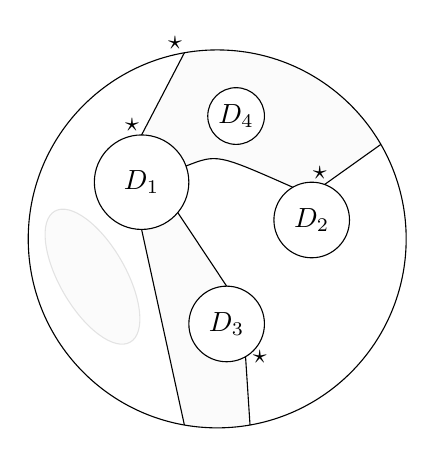
\begin{tikzpicture}[scale=1.2]
			\coordinate (centerO) at (0,0);
			\coordinate (centerA) at (-0.8,0.6);
			\coordinate (centerB) at (1,0.2);
			\coordinate (centerC) at (0.1,-0.9);
			\coordinate (centerD) at (0.2,1.3);
			\def\radiusO{2cm};
			\def\radiusA{0.5cm};
			\def\radiusB{0.4cm};
			\def\radiusC{0.4cm};
			\def\radiusD{0.3cm};
			\def\helligkeit{30};
			
			% shading
			\begin{scope}
				\path[clip] ($(centerO) + (100:\radiusO)$) -- ($ (centerA) +(90:\radiusA) $) --
					($ (centerA) +(90:\radiusA) $) arc [start angle=90 , end angle=20 , radius=\radiusA] --
					($(centerA) + (20:\radiusA)$) .. controls (0,0.9).. ($ (centerB) +(120:\radiusB) $) --
					($ (centerB) +(120:\radiusB) $) arc [start angle=120 , end angle=70 , radius=\radiusB] --
					($ (centerB) +(70:\radiusB) $) -- ($(centerO) + (30:\radiusO)$) --
					($(centerO) + (30:\radiusO)$) arc [start angle=30 , end angle=100 , radius=\radiusO];				
				\fill[color = gray!\helligkeit, opacity=0.1]  (centerO) circle [radius=\radiusO];
			\end{scope}
			
			\begin{scope}			
				\path[clip] ($(centerA) + (-40:\radiusA)$) -- 
					($ (centerC) +(90:\radiusC) $) arc [start angle=90 , end angle=300 , radius=\radiusC] --
					($ (centerC) +(300:\radiusC) $) -- 
					($(centerO) + (-80:\radiusO)$) arc[start angle=-80, end angle=-100, radius=\radiusO] --
					($ (centerA) +(270:\radiusA) $) arc[start angle=270, end angle=320, radius=\radiusA];
				\fill[color = gray!\helligkeit, opacity=0.1]  (centerO) circle [radius=\radiusO];
			\end{scope}
					
			\draw (centerO) circle [radius=\radiusO];
			\draw[fill=white] (centerA) circle [radius=\radiusA];
			\draw[fill=white] (centerB) circle [radius=\radiusB];
			\draw[fill=white] (centerC) circle [radius=\radiusC];
			\draw[fill=white] (centerD) circle [radius=\radiusD];
			
			\draw (centerA) node {$D_1$};
			\draw (centerB) node {$D_2$};
			\draw (centerC) node {$D_3$};
			\draw (centerD) node {$D_4$};	
	
			%strings
			\draw %[decoration={markings, mark=at position 0.3 with {\arrowreversed{triangle 45}}}, postaction={decorate}] 
				($(centerO) + (100:\radiusO)$) -- ($ (centerA) +(90:\radiusA) $);
			\draw %[decoration={markings, mark=at position 0.3 with {\arrowreversed{triangle 45}}}, postaction={decorate}] 
				($(centerO) + (260:\radiusO)$) -- ($ (centerA) +(270:\radiusA) $);
			\draw %[decoration={markings, mark=at position 0.625 with {\arrow{triangle 45}}}, postaction={decorate}] 
				($(centerO) + (30:\radiusO)$) -- ($ (centerB) +(70:\radiusB) $);
			\draw %[decoration={markings, mark=at position 0.625 with {\arrow{triangle 45}}}, postaction={decorate}] 
				($(centerO) + (-80:\radiusO)$) -- ($ (centerC) +(300:\radiusC) $);
			
			\draw %[decoration={markings, mark=at position 0.625 with {\arrowreversed{triangle 45}}}, postaction={decorate}] 
				($(centerA) + (20:\radiusA)$) .. controls (0,0.9).. ($ (centerB) +(120:\radiusB) $);
			\draw %[decoration={markings, mark=at position 0.3 with {\arrowreversed{triangle 45}}}, postaction={decorate}] 
				($(centerA) + (-40:\radiusA)$) -- ($ (centerC) +(90:\radiusC) $);
			
			\draw[fill=gray!\helligkeit, opacity=0.1] (-1.32,-0.4) circle [x radius = 0.35cm, y radius = 0.8cm, rotate = 30];
			
			% marked points
			\node (markedPointO) at ($(centerO) + (100:\radiusO) + (-0.1,0.1)$) {$\markedPoint$};
			\node (markedPointA) at ($(centerA) + (90:\radiusA) + (-0.1,0.1)$) {$\markedPoint$};
			\node (markedPointB) at ($(centerB) + (70:\radiusB) + (-0.05,0.12)$) {$\markedPoint$};
			\node (markedPointC) at ($(centerC) + (-60:\radiusC) + (0.15,0)$) {$\markedPoint$};
		\end{tikzpicture}
		\caption[]{}\label{subfig:TangleFirstExample}
	\end{subfigure}	
	\begin{subfigure}{.49\textwidth}
		\centering
		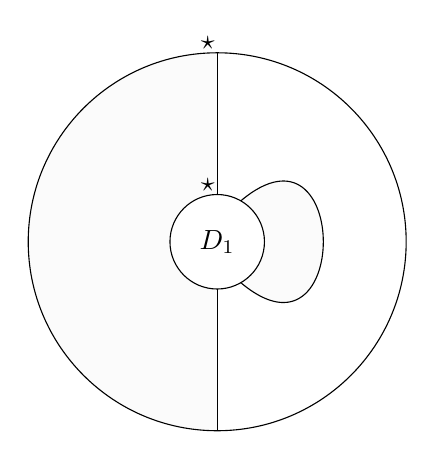
\begin{tikzpicture}[scale=1.2]
			\coordinate (centerO) at (0,0);
			\coordinate (centerA) at (0,0);
			\def\radiusO{2cm};
			\def\radiusA{0.5cm};
			\def\helligkeit{30};
			
			% shading
			\begin{scope}
				\path[clip]
				($ (centerA) +(90:\radiusA) $) arc[start angle=90, end angle=270, radius=\radiusA] --
				($(centerO) + (-90:\radiusO)$) arc[start angle=270, end angle=90, radius=\radiusO];
				\fill[color = gray!\helligkeit, opacity=0.1]  (centerO) circle [radius=\radiusO];
			\end{scope}
			\begin{scope}
				\path[clip] 
					($(centerA) + (60:\radiusA)$) .. controls ($(centerA) + (45:\radiusO)$) and ($(centerA) + (-45:\radiusO)$) .. ($ (centerA) +(-60:\radiusA) $) arc[start angle=300, end angle=60, radius=\radiusA];
				\fill[color = gray!\helligkeit, opacity=0.1]  (centerO) circle [radius=\radiusO];				
			\end{scope}
					
			\draw (centerO) circle [radius=\radiusO];
			\draw[fill=white] (centerA) circle [radius=\radiusA];
			
			\draw (centerA) node {$D_1$};	
	
			%strings
			\draw %[decoration={markings, mark=at position 0.3 with {\arrowreversed{triangle 45}}}, postaction={decorate}] 
				($(centerO) + (90:\radiusO)$) -- ($ (centerA) +(90:\radiusA) $);
			\draw %[decoration={markings, mark=at position 0.3 with {\arrowreversed{triangle 45}}}, postaction={decorate}] 
				($(centerO) + (-90:\radiusO)$) -- ($ (centerA) +(-90:\radiusA) $);		
			\draw %[decoration={markings, mark=at position 0.3 with {\arrowreversed{triangle 45}}}, postaction={decorate}] 
				($(centerA) + (60:\radiusA)$) .. controls ($(centerA) + (45:\radiusO)$) and ($(centerA) + (-45:\radiusO)$) .. ($ (centerA) +(-60:\radiusA) $);		
			
			% marked points
			\node (markedPointO) at ($(centerO) + (90:\radiusO) + (-0.1,0.1)$) {$\markedPoint$};
			\node (markedPointA) at ($(centerA) + (90:\radiusA) + (-0.1,0.1)$) {$\markedPoint$};
		\end{tikzpicture}
		\caption[]{}\label{subfig:CondExp Neg}
	\end{subfigure}
\caption[First examples of planar tangles]{Examples of planar tangles. In (\subref{subfig:TangleFirstExample}) we see a $(4,+)$-tangle whose internal disks have colors $(4,+),(2,-),(2,+),$ and $(0,+)$, respectively. The tangle in (\subref{subfig:CondExp Neg}) is $(2,-)$ with a single internal $(4,-)$ disk.}\label{fig:Tangle Examples1}
\end{figure}

Note that the shading is really only a way of encoding the colors of the disk so that they are easier to recognize. It is not necessary to always draw it. The shading is clear as long as one keeps track of the colors and the marked points of each disk.

\bigno Given an $(n,\epsilon)$-tangle $T$ and an $(\tilde{n},\tilde{\epsilon})$-tangle $S$ such that for some internal disk $D_i$ of $T$ we have $(n_i, \epsilon_i)=(\tilde{n},\tilde{\epsilon})$ we can in a natural way define a new $(n,\epsilon)$-tangle $T\circ_i S$. Namely: plug $S$ into $D_i$ such that the marked and all other distinct points of $S$ and $D_i$ coincide, delete the boundary of $S$, and smooth out the strings. Then 
\begin{align*}
\mathcal{D}_{T\circ_i S} = \left(\mathcal{D}_T- \{D_i\}\right) \cup \mathcal{D}_S,
\end{align*}
and we relabel the internal disks in the obvious way, see \eqref{eq:CompositionInternalDiscs} in the appendix. If there is only one internal disk in which we can insert then we will also drop the index and write $\circ$ instead of $\circ_1$.

We can, for example, $\circ_2$-compose the first tangle in \figref{fig:Tangle Examples1} with the second one and obtain
\begin{center}
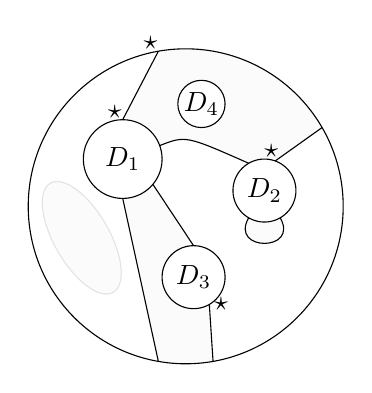
\begin{tikzpicture}[scale=1]
	\coordinate (centerO) at (0,0);
	\coordinate (centerA) at (-0.8,0.6);
	\coordinate (centerB) at (1,0.2);
	\coordinate (centerC) at (0.1,-0.9);
	\coordinate (centerD) at (0.2,1.3);
	\def\radiusO{2cm};
	\def\radiusA{0.5cm};
	\def\radiusB{0.4cm};
	\def\radiusC{0.4cm};
	\def\radiusD{0.3cm};
	\def\helligkeit{30};
	
	% shading
	\begin{scope}
		\path[clip] ($(centerO) + (100:\radiusO)$) -- ($ (centerA) +(90:\radiusA) $) --
			($ (centerA) +(90:\radiusA) $) arc [start angle=90 , end angle=20 , radius=\radiusA] --
			($(centerA) + (20:\radiusA)$) .. controls (0,0.9).. ($ (centerB) +(120:\radiusB) $) --
			($ (centerB) +(120:\radiusB) $) arc [start angle=120 , end angle=70 , radius=\radiusB] --
			($ (centerB) +(70:\radiusB) $) -- ($(centerO) + (30:\radiusO)$) --
			($(centerO) + (30:\radiusO)$) arc [start angle=30 , end angle=100 , radius=\radiusO];				
		\fill[color = gray!\helligkeit, opacity=0.1]  (centerO) circle [radius=\radiusO];
	\end{scope}
	
	\begin{scope}
		\path[clip]
			($(centerB) + (240:\radiusB)$) 
			.. controls ($(centerB) + (240:\radiusB) + (240:0.5cm)$) and ($(centerB) + (300:\radiusB)+(300:0.5cm)$) .. 
			($ (centerB) +(300:\radiusB) $) arc[start angle=-60, end angle=-120, radius=\radiusB];
		\fill[color = gray!\helligkeit, opacity=0.1]  (centerO) circle [radius=\radiusO];
	\end{scope}
	
	\begin{scope}			
		\path[clip] ($(centerA) + (-40:\radiusA)$) -- 
			($ (centerC) +(90:\radiusC) $) arc [start angle=90 , end angle=300 , radius=\radiusC] --
			($ (centerC) +(300:\radiusC) $) -- 
			($(centerO) + (-80:\radiusO)$) arc[start angle=-80, end angle=-100, radius=\radiusO] --
			($ (centerA) +(270:\radiusA) $) arc[start angle=270, end angle=320, radius=\radiusA];
		\fill[color = gray!\helligkeit, opacity=0.1]  (centerO) circle [radius=\radiusO];
	\end{scope}
			
	\draw (centerO) circle [radius=\radiusO];
	\draw[fill=white] (centerA) circle [radius=\radiusA];
	\draw[fill=white] (centerB) circle [radius=\radiusB];
	\draw[fill=white] (centerC) circle [radius=\radiusC];
	\draw[fill=white] (centerD) circle [radius=\radiusD];
	
	\draw (centerA) node {$D_1$};
	\draw (centerB) node {$D_2$};
	\draw (centerC) node {$D_3$};
	\draw (centerD) node {$D_4$};	

		%strings
	\draw %[decoration={markings, mark=at position 0.3 with {\arrowreversed{triangle 45}}}, postaction={decorate}] 
		($(centerO) + (100:\radiusO)$) -- ($ (centerA) +(90:\radiusA) $);
	\draw %[decoration={markings, mark=at position 0.3 with {\arrowreversed{triangle 45}}}, postaction={decorate}] 
		($(centerO) + (260:\radiusO)$) -- ($ (centerA) +(270:\radiusA) $);
	\draw %[decoration={markings, mark=at position 0.625 with {\arrow{triangle 45}}}, postaction={decorate}] 
		($(centerO) + (30:\radiusO)$) -- ($ (centerB) +(70:\radiusB) $);
	\draw %[decoration={markings, mark=at position 0.625 with {\arrow{triangle 45}}}, postaction={decorate}] 
		($(centerO) + (-80:\radiusO)$) -- ($ (centerC) +(300:\radiusC) $);
	
	\draw %[decoration={markings, mark=at position 0.625 with {\arrowreversed{triangle 45}}}, postaction={decorate}] 
		($(centerA) + (20:\radiusA)$) .. controls (0,0.9).. ($ (centerB) +(120:\radiusB) $);
	\draw %[decoration={markings, mark=at position 0.3 with {\arrowreversed{triangle 45}}}, postaction={decorate}] 
		($(centerA) + (-40:\radiusA)$) -- ($ (centerC) +(90:\radiusC) $);
	\draw
		($(centerB) + (240:\radiusB)$) .. controls ($(centerB) + (240:\radiusB) + (240:0.5cm)$) and ($(centerB) + (300:\radiusB)+(300:0.5cm)$) .. ($ (centerB) +(300:\radiusB) $);
	
	\draw[fill=gray!\helligkeit, opacity=0.1] (-1.32,-0.4) circle [x radius = 0.35cm, y radius = 0.8cm, rotate = 30];
	
	% marked points
	\node (markedPointO) at ($(centerO) + (100:\radiusO) + (-0.1,0.1)$) {$\markedPoint$};
	\node (markedPointA) at ($(centerA) + (90:\radiusA) + (-0.1,0.1)$) {$\markedPoint$};
	\node (markedPointB) at ($(centerB) + (70:\radiusB) + (-0.05,0.12)$) {$\markedPoint$};
	\node (markedPointC) at ($(centerC) + (-60:\radiusC) + (0.15,0)$) {$\markedPoint$};
\end{tikzpicture}
\end{center}

This operation of inserting planar tangles into like-colored internal discs of another tangle is called \emph{composition}, and with it we have pretty much already defined the \emph{colored planar operad} $\mathfrak{P}$, see e.g.\ \cite[p 561 f]{loday2012algebraic}.\footnote{If you know about operads then you may see the planar operad as a more `pedantic' version of the \emph{little disks} operad} What this really means is that, for all intents and purposes, we have a collection of things --- in this case, all planar tangles --- and on this collection we define a notion of \emph{composition} that is associative and unital, where `unitality of composition'  means that there are some elements $\id_{(n_i,\epsilon_i)}$ in our collection such that $T\circ_i \id_{(n_i,\epsilon_i)} = T$, whenever this composition is possible.

It is immediately clear what these units are in our case: For fixed $(n,\epsilon)$ they are the unique $(n,\epsilon)$-tangle with exactly one internal $(n,\epsilon)$-disc, and strings only connecting the internal and the external disks s.t.\ both marked points are endpoints of the same string. For example, the following is $\id_{(2,-)}$:
\begin{align*}
\id_{(2,-)} =\,
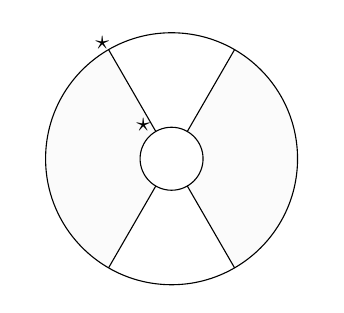
\begin{tikzpicture}[scale=0.8, baseline]
	\coordinate (O) at (0,0);
	\def\radiusO{2cm};
	\def\radiusA{0.5cm};
	\def\helligkeit{30};
%	
	% shading
	\begin{scope}
		\path[clip]
			($ (O) +(120:\radiusO) $) arc[start angle=120, end angle=240, radius=\radiusO] --
			($ (O) +(240:\radiusA) $) arc[start angle=240, end angle=120, radius=\radiusA] ;
		\fill[color = gray!\helligkeit, opacity=0.1]  (O) circle [radius=\radiusO];
	\end{scope}
	\begin{scope}
		\path[clip] 
			($ (O) +(60:\radiusO) $) arc[start angle=60, end angle=-60, radius=\radiusO] --
			($ (O) +(-60:\radiusA) $) arc[start angle=-60, end angle=60, radius=\radiusA] ;
		\fill[color = gray!\helligkeit, opacity=0.1]  (O) circle [radius=\radiusO];				
	\end{scope}
%			
	\draw (O) circle [radius=\radiusO];
	\draw[fill=white] (O) circle [radius=\radiusA];
%
		%strings
	\draw %[decoration={markings, mark=at position 0.3 with {\arrowreversed{triangle 45}}}, postaction={decorate}] 
		($(O) + (120:\radiusO)$) -- ($ (O) + (120:\radiusA) $);
	\draw %[decoration={markings, mark=at position 0.3 with {\arrowreversed{triangle 45}}}, postaction={decorate}] 
		($(O) + (60:\radiusO)$) -- ($ (O) + (60:\radiusA) $);		
	\draw %[decoration={markings, mark=at position 0.3 with {\arrowreversed{triangle 45}}}, postaction={decorate}] 
		($(O) + (-120:\radiusO)$) -- ($ (O) + (-	120:\radiusA) $);
	\draw %[decoration={markings, mark=at position 0.3 with {\arrowreversed{triangle 45}}}, postaction={decorate}] 
		($(O) + (-60:\radiusO)$) -- ($ (O) + (-60:\radiusA) $);		
%	
	% marked points
	\node (markedPointO) at ($(O) + (120:\radiusO) + (-0.1,0.1)$) {$\markedPoint$};
	\node (markedPointA) at ($(O) + (120:\radiusA) + (-0.2,0.1)$) {$\markedPoint$};	
\end{tikzpicture}
\end{align*}
As the symbol already implies it also serves as the identity, since for any $(2,-)$-tangle $T$ we clearly have $\id_{(2,-)} \circ T = T$. 

For $x\in\mathfrak{Col}$ we define $\mathcal{T}_x$ to be the free complex vector space on the set of all planar $x$-tangles. These spaces are often called \emph{$x$-box spaces}\footnotemark, as explained in the following.
Note that $\mathcal{T}_{(n,+)}\cong \mathcal{T}_{(n,-)}$ --- every tangle can be defined with the opposite shading.
\footnotetext{Strictly speaking this name only makes sense for shaded tangles}

\bigno
We promised that there is also a description of tangles in terms of rectangles (or \emph{boxes}) instead of discs. This is sometimes easier, and it surely is easier to draw. To obtain it, simply replace all disks by rectangles (or blow up the disks into rectangles, if you will) so that half of the distinct points is along the top edge and the other half is along the bottom edge, and so that on left of the marked point is a corner of the rectangle.

Then we further impose that in this description the marked point be the left-most point on the top. This can always be done by choosing an appropriate representative of the isotopy class, and it is commonly referred to as the \emph{standard form} of the tangle. It allows us to draw pictures even simpler: The symbol $\markedPoint$ doesn't need to be put next to the marked points anymore, as we now know exactly where they are.

\bigno
In terms of boxes it is now easier to talk about an involution that exists on planar tangles. This involution ${}^*$ yields the \emph{adjoint} $T^*$ of a tangle $T$ as follows.
\begin{itemize}
\item[\textsf{$\bullet$}] Take the tangle in standard form.
\item[$\bullet$] Flip it horizontally, i.e.\ along the horizontal axis.
\item[$\bullet$] Interpret the result as a tangle in standard form --- that is, the point that was the ``last'' point (when enumerating in a clockwise) before the flip is now the marked point.
\item[$\bullet$] Note that this operation reversed the shading. But we want the adjoint to have the same color, so invert the shading.
\end{itemize}
That this is indeed involutive, i.e.\ ${}^{**}=\id$, is an easy exercise.

\bigno
Before we go on, let us list some planar tangles that we will encounter a few times.
\subsection*{A Few Important Tangles}\addcontentsline{toc}{subsection}{A Few Important Tangles}
There are a few tangles that deserve to be mentioned explicitly. All of these tangles can be defined for any box space, so we will only give a few easy examples. Arguably the most important one, the \emph{multiplication tangle}, is given by stacking tangles on top of each other, na\"ively speaking. Its pictorial representation can be found after the definition of planar algebras.

The (second) most important one, which will be used all the time in this thesis, is the \emph{rotation tangle} or \emph{one-click rotation} $\mathsf{rot}:\mathcal{T}_{(n,\pm)}\rightarrow \mathcal{T}_{(n,\mp)}$. An example can be found in \figref{fig:rotation tangle}. Note that what makes it a `rotation' is that the marked point of the internal box is offset by one w.r.t.\ the marked point of the exterior box.

\begin{figure}[!htp]\centering
	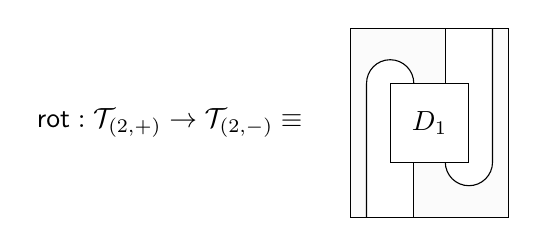
\begin{tikzpicture}
		\node (text) at (-3.3,0) {$\mathsf{rot}:\mathcal{T}_{(2,+)}\rightarrow\mathcal{T}_{(2,-)} \equiv$};
		\def\helligkeit{30};
		\begin{scope}
			\path[clip]
				(-0.2,0.5) arc[start angle=0, end angle=180, radius=3mm] -- ++(0,-1.7) -- ++(-0.2,0) -- ++(0,2.4) -- ++(1.2,0) -- ++(0,-0.7);
			\fill[color = gray!\helligkeit, opacity=0.1]  (-1,-1.2) rectangle (1,1.2);
		\end{scope}
		\begin{scope}
			\path[clip]
				(0.2,-0.5) arc[start angle=180, end angle=360, radius=3mm] -- ++(0, 1.7) -- ++(0.2,0) -- ++(0,-2.4) -- ++(-1.2,0) -- ++(0,0.7);
			\fill[color = gray!\helligkeit, opacity=0.1]  (-1,-1.2) rectangle (1,1.2);
		\end{scope}
		
		\draw[fill= white] (-0.5,-0.5) rectangle (0.5,0.5);
		\node (O) at (0,0) {$D_1$};
		\draw (-1,-1.2) rectangle (1,1.2);
		\draw (-0.2,0.5) arc[start angle=0, end angle=180, radius=3mm] -- ++(0,-1.7);
		\draw (0.2,-0.5) arc[start angle=180, end angle=360, radius=3mm] -- ++(0,1.7);
		\draw (0.2, 0.5) -- ++(0,0.7);
		\draw (-0.2, -0.5) -- ++(0,-0.7);
	\end{tikzpicture}
	\caption[The rotation tangle]{The shaded rotation tangle for $(2,+)$-tangles. All boxes are in standard form. The shading is supplied for clarity.}
	\label{fig:rotation tangle}
\end{figure}

\bigno Now the notation will be getting a bit messy, but we promise that the reader only has to endure this for a short while. We can also define the \emph{inclusion tangle} $\textsf{inc}_{k,\pm}^{k+1}$ (see \figref{fig:InclusionTangle}), which takes a $(k,\pm)$-tangle $S$ and maps it to the $(k+1,\pm)$-tangle $\textsf{inc}_{k,\pm}^{k+1}\circ_1 S$. It of course also makes sense to then define the general symbol $\textsf{inc}_{k,\pm}^{l}\equiv \textsf{inc}_{l-1,\pm}^{l}\circ \ldots \circ \textsf{inc}_{k,\pm}^{k+1}$ for $l>k$, this is just `including the inclusion'.

There also exists a sort of `converse' for the inclusion, commonly called the \emph{conditional expectations tangle} $\mathcal{E}_{k+1,\pm}^{k}$ as seen in \figref{fig:ConditionalExpectationTangle}, taking $(k+1,\pm)$-tangles to $k$-tangles with the same shading for the marked point. For this tangle an obvious generalization $\mathcal{E}_{k+1,\pm}^{l}$, for $l\leq k$, is readily defined.

\begin{figure}[!htp]\centering
	\begin{subfigure}{0.5\textwidth}\centering
		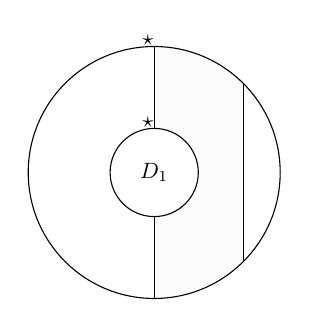
\begin{tikzpicture}[scale=0.8, every node/.style={scale=0.8}]
			\coordinate (centerO) at (0,0);
			\def\radiusO {2cm};
			\def\radiusA {.7cm};
		
			\begin{scope}		
				\path[clip] ($(centerO)+(90:\radiusO)$) -- 
					($(centerO)+(90:\radiusA)$)  arc [start angle=90, end angle=-90, radius=\radiusA] --
					($(centerO) + (-90:\radiusO)$) --
					($(centerO)+(-90:\radiusO)$) arc [start angle=270, end angle=315, radius=\radiusO] --
					($(centerO)+(-45:\radiusO)$) -- 
					($(centerO) + (45:\radiusO)$) arc [start angle=45, end angle=90, radius=\radiusO];	
				\fill[color = gray!30, opacity=0.1]  (centerO) circle [radius=\radiusO];
			\end{scope}
			
			\draw (centerO) circle [radius=\radiusO];
			\draw (centerO) circle [radius=\radiusA];
			\draw ($(centerO)+(90:\radiusO)$) -- ($(centerO)+(90:\radiusA)$);
			\draw ($(centerO)+(-90:\radiusO)$) -- ($(centerO)+(-90:\radiusA)$);
			\draw ($(centerO)+(45:\radiusO)$) -- ($(centerO) + (-45:\radiusO)$);
			\draw (centerO) node {$D_1$};
			
			\draw ($(centerO)+(90:\radiusO) + (-0.1,0.1)$) node {$\markedPoint$};
			\draw ($(centerO)+(90:\radiusA) + (-0.1,0.1)$) node {$\markedPoint$};
		\end{tikzpicture}
		\caption[]{}
		\label{fig:InclusionTangle}
	\end{subfigure}
	\begin{subfigure}{0.49\textwidth}\centering
		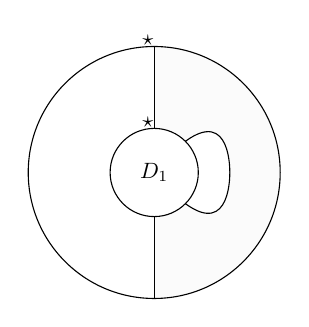
\begin{tikzpicture}[scale=0.8, every node/.style={scale=0.8}]
			\coordinate (centerO) at (0,0);
			\def\radiusO {2cm};
			\def\radiusA {.7cm};		
		
			\begin{scope}		
				\path[clip] ($(centerO)+(90:\radiusO)$) -- 
					($(centerO)+(90:\radiusA)$)  arc [start angle=90, end angle=45, radius=\radiusA] --
					($(centerO)+(45:\radiusA)$) .. 
						controls ($(centerO)+(40:1.6cm)$) and ($(centerO)+(0:1.2cm)$) ..
						($(centerO)+(0:1.2cm)$)..
						controls ($(centerO)+(0:1.2cm)$) and ($(centerO)+(-40:1.6cm)$) ..
						($(centerO)+(-45:\radiusA)$) --
					($(centerO)+(-45:\radiusA)$) arc [start angle=-45, end angle=-90, radius=\radiusA] --
					($(centerO)+(-90:\radiusO)$) arc [start angle=-90, end angle=90, radius=\radiusO];	
				\fill[color = gray!30, opacity=0.1]  (centerO) circle [radius=\radiusO];
			\end{scope}
			
			\draw (centerO) circle [radius=\radiusO];
			\draw (centerO) circle [radius=\radiusA];
			\draw ($(centerO)+(90:\radiusO)$) -- ($(centerO)+(90:\radiusA)$);
			\draw ($(centerO)+(-90:\radiusO)$) -- ($(centerO)+(-90:\radiusA)$);
			\draw ($(centerO)+(45:\radiusA)$) .. 
				controls ($(centerO)+(40:1.6cm)$) and ($(centerO)+(0:1.2cm)$) ..
				($(centerO)+(0:1.2cm)$)..
				controls ($(centerO)+(0:1.2cm)$) and ($(centerO)+(-40:1.6cm)$) ..
				($(centerO)+(-45:\radiusA)$);

			\draw (centerO) node {$D_1$};
			
			\draw ($(centerO)+(90:\radiusO) + (-0.1,0.1)$) node {$\markedPoint$};
			\draw ($(centerO)+(90:\radiusA) + (-0.1,0.1)$) node {$\markedPoint$};
		\end{tikzpicture}
		\caption[]{}
		\label{fig:ConditionalExpectationTangle}
	\end{subfigure}
	
	\caption[Inclusion and conditional expectation tangles]{(\subref{fig:InclusionTangle}) The inclusion tangle $\textsf{inc}_{1,+}^{2}:\mathcal{T}_{(1,+)}\rightarrow\mathcal{T}_{(2,+)}$ and
		(\subref{fig:ConditionalExpectationTangle})	the conditional expectation tangle $\mathcal{E}_{2,+}^{1}$.
	}
\end{figure}

Finally, we can also define another conditional expectation tangle that closes to the left. But observe that this one will switch the shading. We then get two a priori distinct notions of what we call  \emph{trace}, by fixing one of ways of building conditional expectation tangles (i.e.\ closing left or right), and successively applying it until the result lives in either $\mathcal{T}_{(0,+)}$ or $\mathcal{T}_{(0,-)}$.

\bigno\bigno

Before going on to defining planar algebras, let us lose a few words on \emph{unshaded tangles}. The name already suggests the main difference: they do not come with a shading. This means that the set of colors is then really just the set of natural numbers, i.e.\ $\mathfrak{Col} =\mathbb{N}_0$, and we consequently require an unshaded $n$-tangle to have $n$ distinct points on the boundary --- in the shaded case we needed an even number of points so that shading is actually possible. It is clear that then, in general, a representation in terms of boxes is not possible --- only when the number of points is even. 
\subsection{Planar Algebras}
Here, again, we will discuss \emph{shaded planar algebras} first, after which we briefly mention the unshaded case. In the fewest possible words,
\begin{center}
\begin{minipage}{0.8\textwidth}
A shaded planar algebra is an operad homomorphism from $\mathfrak{P}$ to a colored operad $\mathfrak{V}$ of vector spaces.\footnotemark
\end{minipage}
\end{center}
\footnotetext{almost verbatim \cite[Def.\ 2.2]{jones2000planarBipartite}}
That sounds weird, so let us make it more precise. Consider a collection $P\equiv\left\{ P_x \right\}_{x\in\mathfrak{C}}$ of vector spaces, indexed by a set of colors. This collection lives in the symmetric monoidal category $\catname{Vect}_k$ of vector spaces over some field $k$, and we can look at things like
\begin{align*}
\mathrm{Hom}\left( \bigotimes_{x\in U} P_x, P_y\right),\quad \text{for } U\subset\mathfrak{Col},
\end{align*}
i.e.\ linear maps from the tensor product of some of the vector spaces to another vector space in $P$. To discover the operadic structure $\mathfrak{V}$ coming with $P$, we make use of the so-called \emph{tensor-hom adjunction}, which tells us that there is an isomorphism
\begin{align*}
\mathrm{Hom}\left( A\tensor B, C \right)\cong \mathrm{Hom}\left( A,\mathrm{Hom}\left( B,C \right) \right),
\end{align*}
natural in $A, C$ for every $B$ \cite[p 505 f]{aluffi2009algebra} --- basically currying.\footnote{Indeed, the isomorphism may be viewed as
\begin{align*}
A\tensor B \rightarrow C \overset{\sim}{\longleftrightarrow} A\rightarrow\left( B\rightarrow C \right)
\end{align*}
}
Let $U,V\subset \mathfrak{Col}$ be finite, and $x,y\in\mathfrak{Col}$. For any two maps
\begin{align*}
\bigotimes_{a_i\in U} P_{a_i}\morphism{f} P_x \qquad\text{and}\qquad \bigotimes_{b_j\in V} P_{b_j}\morphism{g} P_y,
\end{align*}
there exists a natural composition whenever $x=b_j$. To see this, fix some $l$ s.t.\ $x=b_l$.
By the tensor-hom adjunction there exists a unique map
\begin{align*}
P_x = P_{b_l}  \overset{\tilde{g}}{\dashrightarrow} \mathrm{Hom}\left( \bigotimes_{b\in V-\{b_l\}} P_b, P_y \right)
\end{align*}
corresponding uniquely to $g$. Then we define the composition $g\diamond_l f$ to be the map corresponding to
\begin{align*}
\tilde{g} \circ f \in& \,\mathrm{Hom}\left( \bigotimes_{a_i\in U} P_{a_i}, \mathrm{Hom}\left( \bigotimes_{b\in V-\{b_l\}} P_b, P_y  \right) \right)\\[2em]
\cong& \, \mathrm{Hom}\left(  \bigotimes_{a \in U\cup V-\{b_l\}} P_{a}, P_y\right)
\end{align*}
via the tensor-hom adjunction.
It is now easy to think about what would be considered an `operad homomorphism', and we record this in the following definition.
\begin{definition}[Planar Algebra]\index{Planar Algbra}\label{def:Planar Algebra}
The collection $P$ becomes a planar algebra by choosing an interpretation $Z:\mathfrak{P}\rightarrow\mathfrak{V}$ of planar tangles in terms of linear maps, compatible with the operadic structures.

That is, an $(n,\epsilon)$-tangle $T$ with $k$ internal disks will be mapped to the linear transformation
\begin{align*}
Z(T): \bigotimes_{i=1}^k P_{(n_i,\epsilon_i)} \rightarrow P_{(n,\epsilon)},
\end{align*}
i.e.\ a linear map from the spaces associated with the inner boundaries of the tangle to space associated with the outer boundary. If $k=0$ then the empty tensor product is the underlying field, and $Z(T)$ is therefore a vector in $P_{(n,\epsilon)}$. We also impose $Z(\id_{(n,\epsilon)}) = \id_{(n,\epsilon)}$.

The compatibility is then that $Z$ is something akin to a homomorphism, i.e.\
\begin{align*}
Z(T\circ_i S) = Z(T)\diamond_i Z(S)
\end{align*}
We will also call $P$ itself a planar algebra, and use $Z$ to denote the homomorphism in general.
\end{definition}

We have already implicitly encountered one example. If $P_x = \mathcal{T}_x$ for $x\in\mathfrak{Col}$, then we get an obvious planar algebra structure --- the trivial one --- and can easily see that each $\mathcal{T}_{(n,\epsilon)}$ is turned into an associative algebra with multiplication
\begin{align*}\mathrm{mult}_n \equiv \,
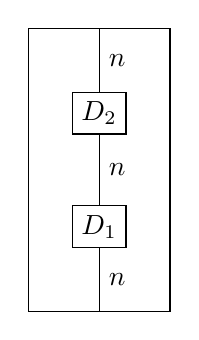
\begin{tikzpicture}[scale=0.9, baseline]
	\coordinate (O) at (0,0);
	\node[draw] (A) at (0,0.8) {$D_2$}; 
	\node[draw] (B) at (0,-0.8) {$D_1$};
	\def\radiusO{2cm};
	\def\radiusA{.6cm};
%
	\draw (-1,-2) rectangle (1,2);
	\draw (0,2) -- node[right] {$n$} (A.north);
	\draw (A.south) -- node[right] {$n$} (B.north);
	\draw (B.south) -- node[right] {$n$} (0,-2);
\end{tikzpicture}\,.
\end{align*}
Here and in the following, an $n$ next to a string implies that there are actually $n$ parallel copies of that string, and the marked points are at the top left of the respective box, as discussed previously. The shading was not drawn, because it is implicitly clear.

The associativity of the multiplication is easily seen by simply remembering  that tangles are defined up to isotopy so that 
\[ \mult_n \circ_1 \mult_n \sim \mult_n\circ_2 \mult_n. \]
Note that this is even commutative if $n=0.$

\subsection*{Additional Stuff, Structure, Property}\addcontentsline{toc}{subsection}{Additional Stuff, Structure, Property}
So far the family of planar $(n,\epsilon)$-tangles is quite large, because there can be an arbitrary collection of closed curves on the inside. Usually, the planar algebras one encounters have an additional property regarding these.

\begin{definition}[Modulus]\index{Modulus!Planar Algebra}
Let $P$ be a planar algebra over $\mathbb{F}$. Let $T$ be a tangle with a closed curve, and let $\hat{T}$ be the same tangle without that curve.

If there exists a
\begin{align*}
\delta \equiv 
\begin{cases}
	\delta_+ &\text{if region bounded by curve is shaded} \\
	\delta_- &\text{if region bounded by curve is unshaded}	
\end{cases}
\in\mathbb{F}
\end{align*}
such that
\begin{align*}
Z(T) = \delta Z(\hat{T})
\end{align*}
then $P$ is said to have \emph{shaded (unshaded) modulus} $\delta_+$ ($\delta_-$). We will only ever encounter the case where $\delta_+ = \delta_->0$, and we then simply say that \emph{$P$ has (positive) modulus $\delta$.}
\end{definition}
\noindent Looking back at the Temperley-Lieb algebras, $\delta$ is also called \emph{loop value}.

\bigno
We may also want to carry the involution on tangles to planar algebras.
\begin{definition}[Planar ${}^*$-algebra]
A planar algebra $P$ over $\mathbb{F}$ is called a \emph{planar ${}^*$-algebra} if $\mathbb{F}$ has a conjugation and if for all colors $x\in\mathfrak{Col}$ the vector space $P_x$ possesses an antilinear involution, such that this involution commutes with the one on planar tangles, that is
\begin{align*}
Z_T(v_1, \ldots, v_k)^* = Z_{T^*}(v_1^*,\ldots, v_k^*)
\end{align*}
for an $n$-tangle $T$ with $k$ internal boxes.
\end{definition}
If the vector spaces are even $C^*$-algebras with that involution, then one speaks of a \emph{planar $C^*$-algebra}.  We only encounter planar algebras consisting of complex vector spaces in this thesis.

The motivation for planar algebras came from the study of subfactors. As famously proven by Jones in \cite[Chapter 4]{jones1999planar1} subfactors give rise to a certain type of planar algebra, and every planar algebra of that type comes from a subfactor. We will now define these important PAs. 
\begin{definition}[Subfactor Planar Algebra]\index{Planar Algebra!Subfactor}
A planar ${}^*$-algebra $S$ is a \emph{subfactor planar algebra} if
\begin{itemize}
\item[\textsf{(i)}] All vector spaces are finite-dimensional, and $\dim S_{0,\pm}=1$. This last property is sometimes called \emph{connectedness}.
\item[\textsf{(ii)}] It is \emph{spherical}: The assignment of complex numbers to labelled\footnotemark\footnotetext{If $T$ is a $(0, \epsilon_0)$-tangle with internal disks $D_i$, then a \emph{labelling} is an element in the range of $Z_T$, drawn as $T$ with some vectors $v_i\in S_{(k_i, \epsilon_i)}$ in the preimage `inserted' into its $i$th internal disk. A labelling is thus equivalently a choice of elements in the domain of $Z_T$.}
 $(0,\pm)$-tangles is invariant under isotopies of the 2-sphere, cf.\ \textsf{Appendix \ref{Appendix:Categories}}. This assignment is called \emph{partition function}. Sphericality means that left and right traces coincide.
\item[\textsf{(iii)}]We can define a positive-definite bilinear form $\langle v,w \rangle\equiv \mathrm{tr}(w^* v)$, which is then called the \emph{inner product}.
\end{itemize}
\end{definition}

A subfactor planar algebra thus has single modulus, as implied by items \textsf{(i)} and \textsf{(ii)}.

\subsection{The Temperley-Lieb Planar Algebra}
The Temperley-Lieb planar algebra $\mathfrak{TL}$ is as simple as it gets, and we can define it as a shaded PA with modulus. All Temperley-Lieb diagrams are already in standard form when interpreted as planar tangles with no internal boxes. It is then clear how to put the two different shadings on a tangle, by simply choosing the color of the first region after the marked point. That way we already get all vector spaces $TL_{(n,\epsilon)}$ whose colors are in $\mathbb{N}\times\{+,-\}$. The two remaining vector spaces $TL_{0,\pm}$ are identified with $\mathbb{C}$.

Tangles with internal boxes act on this collection of vector spaces in an obvious way: TL basis diagrams are tangles, so we just compose and extend by linearity, for each internal disk. Thus by labelling a planar tangle with vectors in TL algebras we get a (multi-)linear map between (products of) these algebras.

Looking back at the definition of subfactor planar algebra, we see that the TL PA almost satisfies it. It has a natural ${}^*$-structure, and the first two items in the definition follow immediately. The inner product, however, need not exist: the bilinear form defined by the trace is not necessarily positive definite, depending on the loop value. Taking quotients by the elements $x$ for which $\langle x,x \rangle=0$ then yields vectors spaces with honest inner products. We can thus turn every Temperley-Lieb planar algebra into a subfactor PA.

We paraphrase \cite{peters2010planar} almost verbatim:
\begin{fact}If $S$ is any subfactor planar algebra with modulus $\delta$, then the obvious `embedding' of the TL PA, i.e.\ the planar algebra homomorphism
\begin{align*}
\mathfrak{TL}\hookrightarrow S,
\end{align*}
given by interpreting Temperley-Lieb tangles as tangles without input disks, is injective if $\delta \geq 2$, otherwise its kernel is the radical of the bilinear form, so that modding out the kernel gives an injective planar algebra homomorphism.
\end{fact}
When we define \emph{perfect tangles} $T$ in the next chapter it will become clear that these are not in the kernel of that map: They are defined such that $\langle T,T \rangle \propto \mathrm{tr}(\mathbf{1_k})$, where $\mathbf{1}_k$ is the tangle that is the multiplicative unit for the multiplication of $k$-tangles.

%\subsection{Instructive Example: The Planar Algebra of a Bipartite Graph}
%Here we will show how, given a bipartite graph, one may construct an associated planar algebra. If one chooses to make this algebra into a planar $*$-algebra, then one obtains a $C^*$-algebra, and we will show how to obtain its Bratelli diagram. \ruggedtodo[inline]{somehow write:} [easy since finite-dimensional $\leadsto$ matrix algebras]


\section{Trivalent Categories}
Trivalent categories, as defined in \cite{Morrison2017Trivalent}, have the nice property that the calculations within are basically calculations in a certain unshaded planar algebra with additional constraints.

We will first write down their category-theoretic definition, but from then on only use string diagrams to apply the methods from the theory of planar algebras. In the vein of the seminal paper we first introduce a few preliminary notions.

The first one is \emph{evaluability}: a monoidal $\mathbb{F}$-linear category is \emph{evaluable} if and only if $\dim\mathrm{Hom}(1,1) = 1$, and that endomorphism space is identified with $\mathbb{F}$ by sending the empty string diagram to $1\in \mathbb{F}$.

Secondly, to rule out a certain degeneracy like before, we call a pivotal category \emph{non-degenerate} iff for every nonzero morphism $f:X\rightarrow Y$ we can find a morphism $f^\prime:Y\rightarrow X$ such that the trace $\mathrm{tr}\left( f^\prime\circ f \right)\in\mathrm{Hom}(1,1)$ is not zero.

For a fixed object $X$ we introduce the notation 
\begin{align*}
\mathcal{C}_n \equiv\mathrm{Hom}\left( 1, X^{\tensor n} \right).
\end{align*}
These vector spaces form an unshaded planar algebra, so far only formally. After the next definition we will understand that $\mathcal{C}_n$ is the span of open planar trivalent graphs with $n$ boundary points, up to isotopy rel boundary, so that only tangles with internal disks of color at most $3$ play any role at all.

\begin{definition}[Trivalent Category]
A triple $\left( \mathcal{C},X,\tau \right)$ forms a \emph{trivalent category} if
\begin{itemize}
\item[•] $\mathcal{C}$ is a strict pivotal $\mathbb{C}$-linear category that is evaluable and non-degenerate
\item[•] $X$ is a self-dual simple object such that 
	\begin{align*}
		\dim\mathcal{C}_1 = 0,\qquad \dim\mathcal{C}_2 = 1,\qquad \dim\mathcal{C}_3 = 1
    \end{align*}
\item[•] $\tau \in \mathcal{C}_3$, called the \emph{trivalent vertex}, is rotationally invariant, that is 
	\begin{align*}
		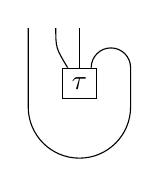
\begin{tikzpicture}[scale=0.5, baseline]
			\node[draw] (t) at (0,0) {$\tau$};
			\foreach \x in {-0.3,0} \draw ($(t.north) + (\x,0)$) .. controls +(\x,0.5) .. ++(\x,1);
		% 
			\draw ($(t.north) + (0.3,0)$) arc[start angle=180, end angle=0, radius=5mm] --
				++ (0,-1) arc[start angle=0, end angle=-180, radius=1.3cm] -- ++ (0,2);
		\end{tikzpicture}
		\, = \,
			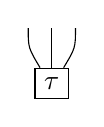
\begin{tikzpicture}[scale=0.5, baseline]
			\node[draw] (t) at (0,0) {$\tau$};
			\foreach \x in {-0.3,0,0.3} \draw ($(t.north) + (\x,0)$) .. controls +(\x,0.5) .. ++(\x,1);
		\end{tikzpicture}\,,
	\end{align*}
	and $\mathcal{C}$ is generated by $\tau$. This means that every morphism is obtained from tensoring and adding identities, (co)evaluations, the self-duality, and trivalent vertices.
\end{itemize}
\end{definition}
Let from now on $\mathcal{C}$ be as in the definition. The object $X$ is actually symmetrically self-dual, meaning that there exists an isomorphism $\phi:X\morphism{\sim} X^*$ with $\phi^* = \phi$. This follows from the non-degeneracy and the dimension of $\mathcal{C}_3$, see Lemma 2.2 in \cite{Morrison2017Trivalent}.

\bigno It is customary to drop the label of the morphism and to simply denote it by a trivalent vertex. Then every string diagram will be an open planar trivalent graph, where strings correspond to simple objects, and two graphs isotopic rel boundary correspond to the same morphism (the self-duality is not drawn). Our category is \emph{defined} to behave nicely, so we can use planar isotopy to deform graphs. For us it is not necessary to reinterpret the graphs as morphisms, since we are only using the graphical calculus.

\bigno Because of the non-degeneracy and the dimensional restrictions we can already extract a few necessary parameters for trivalent categories. For one, any diagram containing the \emph{lollipop}
\begin{align*}
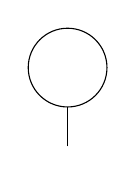
\begin{tikzpicture}[scale=0.5]
	\draw (1,0) arc[start angle=0, end angle=360, radius=1cm];
	\draw (0,-2) -- (0,-1);
\end{tikzpicture}
\end{align*}
as a subgraph is zero, since $\dim\mathcal{C}_1=0$.

Next, a loop (a circle shape) is an element in $\mathbb{C}$, called $d$.  This value must be nonzero, because the loop is the basis element of $\mathcal{C}_2$ composed with its dual.

On the other hand, the following element is in $\mathcal{C}_2$ and must thus be a scalar multiple of the single string,
\begin{align*}

\begin{tikzpicture}[scale=1, baseline]
	\node (A) at (-0.5,-0.8) {};
	\node (B) at (0.5,-0.8) {};
	\foreach \node in {A, B}
		\foreach \x in {-0.3,0,0.3} 
			\draw (\node.north) .. controls +(\x,0.5) .. ++(\x,1);
	\draw ($(A.north) + (0.3,1)$) arc[start angle=180, end angle=0, radius=2mm];
	\draw ($(A.north) + (0,1)$) arc[start angle=180, end angle=0, radius=5mm];
	\draw ($(A.north) + (-0.3,1)$) -- ++(0,0.5);
	\draw ($(B.north) + (0.3,1)$) -- ++(0,0.5);
\end{tikzpicture} \, = \, b\cdot \,

\begin{tikzpicture}[baseline]
	\draw (-0.5,0.3) arc[start angle=180, end angle=360, radius=5mm];
\end{tikzpicture}\,,
\end{align*}
and like before putting a cap on this must yield $bd\neq 0$, so the parameter $b$  must be nonzero. The trivalent vertex can be normalized so that we always take $b=1$.

Finally, we can rotate and compose trivalent vertices such that the result lives again in $\mathcal{C}_3$ (just imagine all legs bent up), and it must thus be some multiple of the trivalent vertex itself, like so:
\begin{align*}
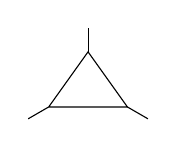
\begin{tikzpicture}[baseline]
	\coordinate (a) at (0,0.5);
	\coordinate (b) at (-0.5,-0.2);
	\coordinate (c) at (0.5,-0.2);
	\draw (a) -- ++ (0,0.3);
	\draw (b) -- ++(210:3mm);
	\draw (c) -- ++(330:3mm);
	\path[draw] (b) -- (a) -- (c) -- (b);
\end{tikzpicture}\, = t\cdot \,
\begin{tikzpicture}[baseline]
	\foreach \angle in {90, 210, 330}
		\draw (0,0) -- ++(\angle:5mm);
\end{tikzpicture}.
\end{align*}
However, coming from the composition, $t$ could actually vanish here.

\bigno In their paper, Morrison \emph{et al} then started classifying trivalent categories by
\begin{itemize}
\item[\text{a)}] the dimensions of the morphism spaces $\mathcal{C}_n$, together with
\item[\text{b)}] the parameters $d$ and $t$, often satisfying some polynomial unique to the category.
\end{itemize}

In this paper, we only look at trivalent categories where $\dim\mathcal{C}_4$ is 4-dimensional, and a basis is provided by the set of all planar trivalent graph with 4 four boundary points and no internal faces. Any trivalent category with this property is called a \emph{cubic category}.

Cubic categories have a nice relation for the square (the trivalent graph with four boundary points, four trivalent vertices, and one internal face), and that makes them particularly nice to work with.

\bigno
It is clear how to interpret open trivalent graphs with $n$-boundary points as unshaded $n$-tangles: We only need to agree on the marked points, and blow up each trivalent vertex to an internal $3$-disk, labelled with $\tau$, and we also simply call that disk $\tau$. \emph{Rotational invariance} then means $\mathrm{rot}\tau = \tau$, so the choice of marked point on $3$-disks doesn't actually matter at all.

A caveat is appropriate here: In planar algebras, we used the symbol ${}^*$ do denote the adjoint or dual of a tangle. That symbol, however, is already reserved in trivalent categories for the category-theoretic dual. Thus for a morphism $f$ in a trivalent category, $f^*$ means ``rotate through $\pi$''. Luckily, it is quickly checked that the notion of horizontally reflecting morphisms is just an instance of what has been called \emph{conjugation} before, for example in \cite{wang2010topological}, where conjugation of morphisms $f,g$ in a pivotal $\mathbb{C}$-linear category was defined as an anti-linear operation $\overline{\phantom{f}}$ that switches source and target of a morphism and satisfies
\begin{align*}
\overline{\overline{f}} = f,\qquad\qquad \overline{f\tensor g} = \overline{f}\tensor\overline{g},\qquad\qquad \overline{f\circ g} = \overline{g}\circ \overline{f}.
\end{align*}
Keeping that in mind, translating the following discussion of \emph{perfect tangles} to trivalent categories is then but a quick change in notation.


\section{Perfect Tangles: Definition and Examples}
	In this chapter we will get to the heart of this thesis, and finally generalize (planarly) perfect tensors to planar algebras. Most of the definitions will be for planar algebras which are (implicitly) shaded, i.e.\ we only consider tangles with an even number of marked points, as they are far easier to handle. And of course, shaded planar algebras are a subset of unshaded ones in a certain way --- that means examples found in the shaded case will work just as well for the unshaded case.

After defining \emph{perfect tangles}, we will see a a few ways of constructing `larger' perfect tangles from `smaller' ones. The first of these was hinted at by Jones, subsequent results were found applying a similar strategy, but it is not yet entirely clear why this strategy seems to work: One uses braid-infused heuristics to draw pictures and translates these into the language of planar tangles. In the special case of the Temperley-Lieb planar algebra this is justified, since perfect tangles give rise to a unitary representation of the braid group, as we will show --- but for general labelled tangles the proof of the Yang-Baxter equation, i.e.\ the third Reidemeister move, is not clear. Something similar to this braiding has already been seen in \cite[Theorem 2.11.3]{jones1999planar1}.

Because of how our definitions and proofs work, this is applicable to perfect tensors as well, so in particular the constructions yield tensor networks with an even number of open edges such that inserting a perfect tensor at each vertex will result in the evaluated tensor network being perfect --- planarly, of course.

\bigno After that we will give a few explicit examples that have been found with the aid of an open source computer algebra system, \texttt{sage}, and Mathematica. Unfortunately, the amount of equations one has to solve is fairly large --- and they are all quadratic, with a lot of variables. The resulting high computational cost prevented the efficient discovery of more than a few examples. But there's still some hope, as some examples can be obtained by directly applying the general constructions to already known smaller perfect tangles.

\section{Perfect Tangles in Planar Algebras}
Our approach is fairly simple, and may readily be seen as some sort of generalization of \emph{biunitaries}, as defined in \cite[p.\ 54 ff.]{jones1999planar1}. Biunitaries, however, are a bit more restricted. Despite them being perfect, not every perfect tangle of the appropriate color is a biunitary in the sense of Jones.

As before, we shall only look at planar algebras with modulus. While it is certainly easier to proceed the way we will --- defining this only for unshaded planar algebras --- one must keep the subtleties that come with substituting `unshaded' with `shaded' in mind, e.g.\ rotating the multiplicative unit by one click swaps the shading, or the fact that the loop values for $\circ$ and {$\bullet$} might be different (this, however, only changes the proportionality factor, and in general we assume that all planar algebras have a single positive modulus).

\bigno The setting is now in some unshaded planar algebra, say $P$, but we will only regard boxes with an even number of distinct boundary points, i.e.\ a shaded planar algebra where, roughly speaking, the shading does not make a difference.

\begin{definition}[Rotated Multiplication]\index{Rotated Multiplication}
Consider $2k$-boxes. For ${0\leq n < 2k}$
we define the \emph{rotated multiplications}
\begin{align*}
\rotatedmultiplication{n}\equiv \mult_k \circ \left( \rot^n,\rot^{-n} \right),
\end{align*}
written as an infix, that is
\begin{align*}
T \rotatedmultiplication{n} S = \rot^n(T)\cdot \rot^{-n}(S).
\end{align*}
Note that a negative exponent on $\rot$ means \emph{clockwise rotation}.
\end{definition}

The rotated multiplication has a rather interesting property. To express this property in a fairly condensed fashion, we can analogously define something like $\stackrel{m}{\curvearrowright}$, where the first argument is rotated clockwise and the second one counterclockwise.

\begin{proposition}\label{Prop:ROT INVROT}
Let $T\in P_{2k}$. Then the following are equivalent.
\begin{itemize}
\item[(i)] $\forall 0\leq n <2k:\quad T \rotatedmultiplication{n} T^* \propto\mathbf{1}_k$
\item[(ii)] $\forall 0\leq n <2k:\quad T^* \stackrel{n}{\curvearrowright} T \propto\mathbf{1}_k$,
\end{itemize}
where $\mathbf{1}_k$ is the is the multiplicative unit.

\normalfont This should not come as a surprise, and the crucial insight only comes in the proof.
\begin{proof}
First, let $0\leq n < k$. Then
\begin{align*}
	T\rotatedmultiplication{n}T^* &= \,
	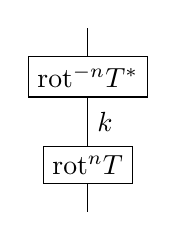
\begin{tikzpicture}[scale = 0.7, baseline=-1mm]
		\node[draw] (T) at (0,-0.8) {$\mathrm{rot}^n T$};
		\node[draw] (Tdag) at (0,0.8) {$\mathrm{rot}^{-n} T^*$};
		\draw (T.south) -- ++ (0,-0.5);
		\draw (Tdag.north) -- ++ (0,0.5);
		\draw (T.north) -- node[right]{$k$} (Tdag.south);
	\end{tikzpicture} = \,
	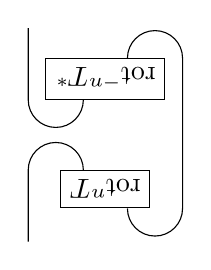
\begin{tikzpicture}[scale = 0.7, baseline=-1mm]
		\node[draw,rotate=180] (T) at (0,-1) {$\mathrm{rot}^n T$};
		\node[draw,rotate=180] (Tdag) at (0,1) {$\mathrm{rot}^{-n} T^*$};
		\draw ($(T.south)+(-0.4,0)$) arc[start angle=0, end angle=180, radius=5mm] -- ++(0,-1.3);
		\draw ($(Tdag.north)+(-0.4,0)$) arc[start angle=0, end angle=-180, radius=5mm] -- ++ (0,1.3);
		\draw ($(Tdag.south)+(0.4,0)$) arc[start angle=180, end angle=0, radius=5mm] -- 
			($(T.north)+(1.4,0)$) arc[start angle=0, end angle=-180, radius=5mm];
	\end{tikzpicture}\\
	&=\,
	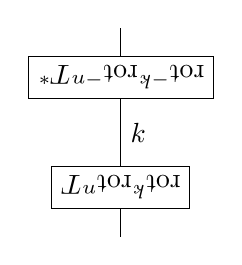
\begin{tikzpicture}[scale = 0.7, baseline=-1mm]
		\node[draw,rotate=180] (T) at (0,-1) {$\mathrm{rot}^k\mathrm{rot}^n T$};
		\node[draw,rotate=180] (Tdag) at (0,1) {$\mathrm{rot}^{-k}\mathrm{rot}^{-n} T^*$};
		\draw (T.north) -- ++ (0,-0.5);
		\draw (Tdag.south) -- ++ (0,0.5);
		\draw (T.south) -- node[right]{$k$} (Tdag.north);
	\end{tikzpicture}\\
	&= \mathrm{rot}^k\left( \mathrm{rot}^{-(k+n)} T^*\cdot \mathrm{rot}^{k+n}T \right) \\
	&= \mathrm{rot}^k\left( T^* \stackrel{k+n}{\curvearrowright} T \right)
\end{align*}
Thus for all $0\leq n < k$:
\begin{align*}
T\rotatedmultiplication{n}T^* \propto \mathbf{1}_k \quad \iff\quad T^*  \stackrel{k+n}{\curvearrowright} T\propto \mathbf{1}_k,
\end{align*}
and one similarly shows
\begin{align*}
T\rotatedmultiplication{k+n}T^* \propto \mathbf{1}_k \quad \iff\quad T^*  \stackrel{n}{\curvearrowright} T\propto \mathbf{1}_k.
\end{align*}
Because $\mathrm{rot}^{2k} = \id$ and $\mathrm{rot}^n\mathrm{rot}^m = \mathrm{rot}^{n+m}$, we finally obtain for all $0\leq n< 2k$
\begin{align*}
T\rotatedmultiplication{n}T^* \propto \mathbf{1}_k \quad \iff\quad T^*  \stackrel{k+n}{\curvearrowright} T\propto \mathbf{1}_k.
\end{align*}
\end{proof}
\end{proposition}
To draw these diagrams this way we used the simple fact that $ \mathrm{rot}_k^n(T) ^* = \left(\mathrm{rot}_k^n\circ T\right)^*= \left(\mathrm{rot}_k^n\right)^*\circ T^*=\mathrm{rot}_k^{-n}\left( T^* \right)$.

\begin{definition}[Perfect Tangle]\label{def:Perfect Tangle}
Let $T\in P_{2k}$. $T$ is called a \emph{perfect $k$-tangle} if for $0\leq n < k$
\begin{align*}
T \rotatedmultiplication{n} T^* \propto T^* \stackrel{n}{\curvearrowright} T \propto \mathbf{1}_k
\end{align*}

As an illustrating example we refer to \figref{fig:Perfect Tangle Condition}. $T$ might also be called a \emph{rotation-invariant unitary} or \emph{a k-unitary}, in analogy with the term \emph{biunitary}.
\end{definition}
The name comes from the first examples found in Temperley-Lieb, where $T$ is actually an honest planar tangle. Note that perfect $k$-tangles are `even' and live in $P_{2k}$. This is just \emph{compression of information}.
In the future we will refer to any $x\in P_k$ as a tangle because $x=Z(\mathrm{id}_k)(x)$, i.e.\ it is a \emph{labelled tangle}.

\begin{figure}[!htp]\centering
	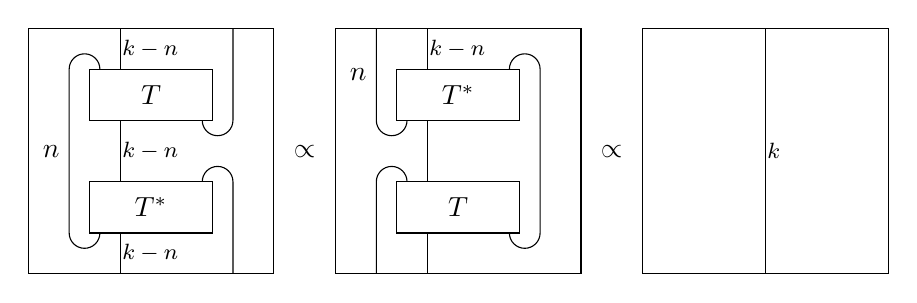
\begin{tikzpicture}[scale=1.3]
		\begin{scope}
			\coordinate (center) at (0,0);
			\draw ($(center) + (-1.2,1.2)$) rectangle ($(center) + (1.2,-1.2)$);
			\draw ($(center) + (-0.6,0.8)$) rectangle ($(center) + (0.6,0.3)$);
			\draw ($(center) + (-0.6,-0.8)$) rectangle ($(center) + (0.6,-0.3)$);

			\node (T) at ($(center) + (0,0.55)$) {$T$};
			\node (TStar) at ($(center) + (0,-0.55)$) {$T^*$};
			
			\draw ($(center) + (-0.5,0.8)$) arc [start angle = 0, end angle= 180, radius=1.5mm] -- node[midway, left] {$n$} 
					($(center) + (-0.8,-0.8)$) arc [start angle = 180, end angle=360, radius=1.5mm];
			\draw ($(center) + (0.5,0.3)$) arc [start angle = 180, end angle=360, radius=1.5mm] --
					($(center) + (0.8,1.2)$);
			\draw ($(center) + (0.5,-0.3)$) arc [start angle = 180, end angle=0, radius=1.5mm] --
					($(center) + (0.8,-1.2)$);
					
			\draw ($(center) + (-0.3,0.8)$) -- ($(center) + (-0.3,1.2)$) node [midway, right] {\hspace*{-1mm}\footnotesize $k-n$};
			\draw ($(center) + (-0.3,-0.8)$) -- ($(center) + (-0.3,-1.2)$) node [midway, right] {\hspace*{-1mm}\footnotesize $k-n$};
			\draw ($(center) + (-0.3,-0.3)$) -- ($(center) + (-0.3,0.3)$) node [midway, right] {\hspace*{-1mm}\footnotesize $k-n$};
		\end{scope}
		\node (propto) at (1.5,0) {$\propto$};
		\begin{scope}
			\coordinate (center) at (3,0);
			\draw ($(center) + (-1.2,1.2)$) rectangle ($(center) + (1.2,-1.2)$);
			\draw ($(center) + (-0.6,0.8)$) rectangle ($(center) + (0.6,0.3)$);
			\draw ($(center) + (-0.6,-0.8)$) rectangle ($(center) + (0.6,-0.3)$);

			\node (T) at ($(center) + (0,0.55)$) {$T^*$};
			\node (TStar) at ($(center) + (0,-0.55)$) {$T$};
			
			\draw ($(center) + (0.5,0.8)$) arc [start angle = 180, end angle= 0, radius=1.5mm] -- 
					($(center) + (0.8,-0.8)$) arc [start angle = 360, end angle=180, radius=1.5mm];
			\draw ($(center) + (-0.5,0.3)$) arc [start angle = 360, end angle=180, radius=1.5mm] -- node[midway, left] {$n$} 
					($(center) + (-0.8,1.2)$);
			\draw ($(center) + (-0.5,-0.3)$) arc [start angle = 0, end angle=180, radius=1.5mm] --
					($(center) + (-0.8,-1.2)$);
					
			\draw ($(center) + (-0.3,0.8)$) -- ($(center) + (-0.3,1.2)$) node [midway, right] {\hspace*{-1mm}\footnotesize $k-n$};
			\draw ($(center) + (-0.3,-0.8)$) -- ($(center) + (-0.3,-1.2)$) node [midway, right] {};
			\draw ($(center) + (-0.3,-0.3)$) -- ($(center) + (-0.3,0.3)$) node [midway, right] {};
		\end{scope}
		\node (propTO) at (4.5,0) {$\propto$};
		\begin{scope}
			\coordinate (center) at (6,0);
			\draw ($(center) + (-1.2,1.2)$) rectangle ($(center) + (1.2,-1.2)$);
			\draw  ($ (center) + (0,-1.2)$)  -- ($ (center) + (0,1.2)$) node [midway, right] (TextNode) {\hspace*{-1mm}\footnotesize $k$};
		\end{scope}
	\end{tikzpicture}
	\caption[Definition of perfect planar tangle]{The defining condition a $k$-tangle $T$ has to satisfy to be perfect}
	\label{fig:Perfect Tangle Condition}
\end{figure}

\bigskip \noindent Before justifying this definition we first introduce new families of diagrams.

\begin{definition}[$(m\rightarrow n)$-family]
Let $T$ be a $k$-tangle. We will call the strings emanating from boundary of the internal (labelled) box the \emph{legs} of $T$. A $k$-tangle thus has $k$ legs, which we can partition into two connected collections with cardinalities $n$ and $m$, respectively, such that $n+m=k$. We do not lose generality when we stipulate $1\leq m\leq n$.

Now, take a partition where the $m$ legs are along the bottom boundary (w.r.t.\ the marked point) of $T$, without loss starting at the leftmost point. The remaining $k-m$ legs along the bottom are bent upwards, i.e.\ isotoped so that they `point in the same direction' as the legs along the top. The result is surrounded by a (dotted) box with $n$ points on the top, $m$ points on the bottom.

This procedure, applied to all rotations of $T$, generates all such boxes that may be obtained from $T$, which we then collect into the so-called \emph{$(m\rightarrow n)$-family} of $T$, also denoted $T[m\rightarrow n]$. The motivation behind the arrow is: Read the tangle as flowing from the bottom to the top.

The dual construction then yields the families $T^*[n\rightarrow m]$ by simple applying ${}^*$ to $T[m\rightarrow n]$, or rotating $T^*$ clockwise, then bending the obvious legs down.

This definition is then extended linearly.
\end{definition}
\begin{figure}[!htp]\centering
	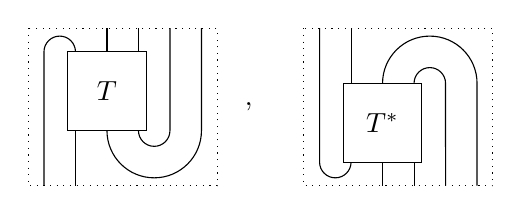
\begin{tikzpicture}
		\node (T) at (0,0) {$T$};
		\draw (-0.5,0.5) rectangle (0.5,-0.5);
		\foreach \x in {0,0.4}
			\draw (\x, 0.5) -- (\x,0.8);
		\draw (-0.4,-0.5) -- (-0.4,-1.2);
		\draw (-0.4,0.5) arc [start angle=0, end angle=180, radius=2mm] -- (-0.8,-1.2);
		\draw (0.4,-0.5) arc [start angle=180, end angle=360, radius=2mm] -- (0.8,0.8);
		\draw (0,-0.5) arc [start angle=180, end angle=360, radius=6mm] -- (1.2,0.8);				
		\draw[dotted] (-1,0.8) rectangle (1.4,-1.2);
		
		\node (comma) at (1.8, -0.2) {,};
		
		\node (TStar) at (3.5,-0.4) {$T^*$};
		\draw (3,0.1) rectangle (4,-0.9);
		\foreach \x in {3.5,3.9}
			\draw (\x, -0.9) -- (\x,-1.2);
		\draw (3.5-0.4,0.1) -- (3.5-0.4,0.8);
		\draw (3.5-0.4,-0.9) arc [start angle=0, end angle=-180, radius=2mm] -- (3.5-0.8,0.8);
		\draw (3.5+0.4,0.1) arc [start angle=180, end angle=0, radius=2mm] -- (3.5+0.8,-1.2);
		\draw (3.5 + 0,0.1) arc [start angle=180, end angle=0, radius=6mm] -- (3.5+1.2,-1.2);				
		\draw[dotted] (2.5,0.8) rectangle (4.9,-1.2);
	\end{tikzpicture}
	\caption[Bending the legs]{An element of $T[2\rightarrow 4]$ and its dual, for a $6$-tangle $T$. This one is essentially the result of first rotating $T$ by one click, then applying the procedure.}
\end{figure}
Multiplication $\alpha\cdot \beta$ of $\alpha\in T[m\rightarrow n]$ with $\beta\in T^*[n\rightarrow m]$ is given by stacking $\beta$ on top of $\alpha$, resulting in a proper $m$-tangle.

\begin{lemma}
If $T\in P_{2k}$ is a perfect $k$-tangle, then for all $\alpha\in T[m\rightarrow n]$ with $m<k$ we have $\alpha\cdot \alpha^* \propto \mathbf{1}_m$.
\begin{proof}
It is clear that $A=\alpha\cdot\alpha^*$ is an $m$-tangle. We can uniquely surround the boxes in $A$ by another box such that the result is a $k$-tangle $\mathcal{T}$, satisfying 
\begin{align*}
A = \mathcal{E}^m_k\left( \mathcal{T} \right).
\end{align*}
It follows from the construction of $T[m\rightarrow n]$ that there is an $ 0\leq l < k$ such that $\alpha$ is `generated' by $\mathrm{rot}^l_k(T)$.
Clearly we thus have
\begin{align*}
A &= \mathcal{E}^m_k\left( \mathcal{T} \right)\\
&= \mathcal{E}^m_k\left(  \mathrm{rot}^l_k(T)\cdot \mathrm{rot}^{-l}_k\left( T^* \right)  \right)\\
&= \mathcal{E}^{m}_k\left( T\rotatedmultiplication{l}T^* \right)\\
&= \mathcal{E}^m_k \left( \lambda\mathbf{1}_k \right)\\
&\propto  \mathbf{1}_m
\end{align*}
The proportionality in the last line is given by a function of the loop values.
\end{proof}
\end{lemma}

A picture might help clarifying this proof. Here the dotted rectangle is the lower half of the box we surrounded $\alpha\cdot\alpha^*$ with in the proof, for $\alpha$ the $T[2\rightarrow 4]$ element from above:
%\begin{figure}[!htp]\centering
	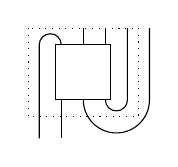
\begin{tikzpicture}[scale=0.7,baseline=-1ex]
		\draw (-0.5,0.5) rectangle (0.5,-0.5);
		\foreach \x in {0,0.4}
			\draw (\x, 0.5) -- (\x,0.8);
		\draw (-0.4,-0.5) -- (-0.4,-1.2);
		\draw (-0.4,0.5) arc [start angle=0, end angle=180, radius=2mm] -- (-0.8,-1.2);
		\draw (0.4,-0.5) arc [start angle=180, end angle=360, radius=2mm] -- (0.8,0.8);
		\draw (0,-0.5) arc [start angle=180, end angle=360, radius=6mm] -- (1.2,0.8);				
		\draw[dotted] (-1,0.8) rectangle (1,-0.8);
	\end{tikzpicture}
%\end{figure}

Note that this lemma tells us: You only need to calculate the products for all $2k$ elements of $T[k\rightarrow k]$, i.e.\ all rotations of $T$. Everything else follows. Thus this definition of perfect tangle is indeed a good generalization of the notion of planarly perfect tensor, in that it captures the isometric properties of \emph{all} planar bipartitions. 

In particular this is the argument for not working in the Temperley-Lieb category, where objects are natural numbers and we more or less have $\mathrm{Hom}(n,m) = T[n\rightarrow m].$ Working with standard TL-diagrams is sufficient.

~\\
\begin{remark}
But we are also interested in finding perfect tangles in trivalent categories. To distinguish them, we shall call them \emph{perfect morphisms}. Remembering the definition of perfect tensors, it is relatively easy to define perfect $(2n+1)$-tangles. We only need to define a multiplication like the \emph{rotated multiplication} --- where the lower (upper) disk has $n+1$ legs bent up (down), and rotation is given like before. $n+1$ is exactly $\ceil{\frac{2n+1}{2}}$, i.e.\ the smallest integer larger than half the number of boundary points.

This can be justified similarly to the previous lemma.

So far, we did not find odd perfect morphisms aside from the obvious one, the trivalent vertex itself. Thus not a lot is known about these, and we will only briefly mention them.
\end{remark}

\section{Simplifications in the Temperley-Lieb Planar Algebra}
As mentioned before, we will mostly be working in the TL planar algebra. We thus need to discuss  the complexity of the calculations and how to reduce it, if possible. 

The amount of equations obtained from computing all products of all $2n$ rotations of a general Temperley-Lieb $n$-tangle is rather frightening. Indeed, if the coefficients are assumed to be complex, then the number of (real) variables is $2$ times the dimension, i.e.\
\begin{align*}
2 C_n = 2 \cdot \frac{1}{n+1}\binom{2n}{n},
\end{align*}
\begin{sagesilent}
output_str = r""
for i in range(1,6):
    answer = 2*catalan_number(i)
    output_str += r"$%s$, "%(answer)

answer = 2*catalan_number(6)
output_str += r"$%s$"%(answer)
\end{sagesilent}
hence the first few numbers read \sagestr{output_str}. The equations are the coefficients of the vectors (in the product) unequal to the unit, together with the inequality $\alpha \neq 0$, where $\alpha$ is the coefficient of the unit. The maximum number of (complex) equations is then \emph{dimension times rotations} $= 2 n\cdot C_n$, which obviously grows very quickly

\bigno Luckily, we can reduce this a bit. In $TL_n$ there are no extra relations for the tangles, it is the \emph{free} vector space on the appropriate set. It is thus necessary that a perfect tangle have support on $\mathbf{1}_n$, which allows us to normalize so that the coefficient of $\mathbf{1}_n$ is of modulus $1$. We will for the sake of simplicity and without loss of generality set $\alpha=1$. This already reduces the number of coefficients by $2$.\footnote{But beware: This does not work in other situations, like trivalent categories for example.}

 We could also only look, say, at rotation invariant tangles, i.e.\ $n$-tangles $T$ with $\rot(T)=T$. We then only have to compute $T\cdot T^*$ and find solutions to get perfect tangles. Moreover, since the coefficient of the unit is normalized to $1$, coefficients of all rotations also have to be $1$, effectively reducing the number of coefficients by more than $n-1$. Then
 \begin{align*}
 \# \text{unknowns} < 2(C_n - n), \qquad  \# \text{equations}  < C_n - n,
 \end{align*}
 i.e.\ solving this problem is already a lot easier.
 
Of course, a logical approach is also to look only at self-adjoint tangles, that is tangles $T$ with $T^* = T$. At the very least the generators of $TL_n$ (of which there are $n-1$, cf.\ our first discussion of the Temperley-Lieb algebras) are self-adjoint, so that their respective coefficients have to be real.

Combining both of these approaches is possible as well, and they are implemented in the code (see \textsf{Appendix \ref{App: Code}} and the code for details).

\bigno Another thing one might hope to succeed is looking at $n$-tangles that are eigenvectors of rotation with eigenvalue a primitive $(2n)$th root of unity, that is
\begin{align*}
\rot T  = e^{\frac{2\pi i}{2n}}T.
\end{align*}
However, in the following lemma we proof that these don't exist in the Temperley-Lieb case.

\begin{lemma}
Let $T\in TL_n$. If
\begin{align*}
\rot  T  = e^{\frac{2\pi i}{2n}}T,
\end{align*}
then $T$ is not perfect.
\begin{proof}
Suppose $T$ is an $n$-tangle with that property, and assume that it is perfect. Note that is then has support on $\mathbf{1}_n$. Then
\begin{align*}
\rot^n T =& \left( e^{\frac{\pi i}{n}} \right)^n T \\
=& e^{i\pi} T \\
=& -T.
\end{align*}
But $\rot^n \mathbf{1}_n = \mathbf{1}_n$,  contradicting $T = -T$.
\end{proof}
\end{lemma}

\section{On the Support of Perfect Temperley-Lieb Tangles}
Later, when we encounter examples of our first general construction, we can observe that all tangles obtained this way seem to have full support, i.e.\ they have nonzero coefficients for all tangles in the standard basis.

We will now make a few observations that hint at this being true for any perfect tangle in Temperley-Lieb, which would of course mean that a perfect tangle in $TL_n$ would be a sum of $\dim TL_n$ terms. A proof, however, is not being provided.

\bigno The statement is trivially true for $n=2$, and the $3$-strand case follows the same procedure as the others, but is not as interesting. We will mainly focus on $TL_4$, but a few observations can be made for arbitrary $n$.

We write $\supp T$ for the support of a tangle $T$. From the definition of \emph{perfectness} and because 
\begin{align*}
1_n \in \supp{\left( TT^* \right)} \iff 1_n \in \supp T
\end{align*}
we can immediately extract that 
\begin{align*}
T\text{ is perfect } \implies \{\rot^l 1_n : 0\leq l < n\}\subseteq \supp T.
\end{align*}
One then might naively guess the inclusion is actually a proper equality for some tangles, but for all cases other than $n=2$ this will not work. Observe first that
\begin{align*}
\rot^l 1_n = 
\begin{cases}
	\quad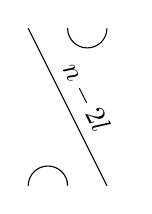
\begin{tikzpicture}[scale = 0.5, baseline]
		\draw (-1,2) -- node[above, sloped]{$n-2l$} (1,-2);
		\draw (0,2) arc[start angle=180, end angle=360, radius=5mm];
		\draw (-1,-2) arc[start angle=180, end angle=0, radius=5mm];
	\end{tikzpicture}
	&\quad l < \ceil{\frac{n}{2}},\\[3.5em]
	\hspace*{1.03mm}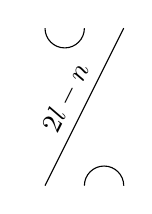
\begin{tikzpicture}[scale = 0.5, baseline]
		\draw (-1,-2) -- node[above, sloped]{$2l-n$} (1,2);
		\draw (0,-2) arc[start angle=180, end angle=0, radius=5mm];
		\draw (-1,2) arc[start angle=180, end angle=360, radius=5mm];
	\end{tikzpicture}
	&\quad l \geq \ceil{\frac{n}{2}},
\end{cases}
\end{align*}
whence 
\begin{align*}
\rot^l 1_n \cdot \rot^{-k} 1_n \propto\,
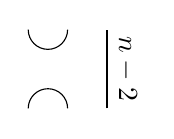
\begin{tikzpicture}[scale=0.5, baseline=-1mm]
	\draw (-1,1) arc[start angle=180, end angle=360, radius=5mm];
	\draw (-1,-1) arc[start angle=180, end angle=0, radius=5mm];
	\draw (1,-1) -- node[above, sloped, rotate=180] {$n-2$} (1,1);
\end{tikzpicture}
\quad \iff \quad k = l = 1.
\end{align*}
But this means: If $T$ has support only on the rotations of $1_n$, and if we label the coefficient of $\rot 1_n$ in $T$ $\alpha$, then there will be a term whose support is $q\lvert \alpha \rvert^2$ times the basis tangle $S$ which is proportional to $\rot 1_n \cdot \rot\inv 1_n$. So if $T$ were perfect, $\alpha$ would have to vanish, contradicting the fact that $T$ has support on $\rot 1_n$. Therefore, $T$ cannot be perfect.

In other words
\begin{align*}
T\text{ is perfect } \implies \{\rot^l 1_n : 0\leq l < n\}\subsetneq \supp T.
\end{align*}

So we have to include all tangles that are rotations of the first generator of Temperley-Lieb as well. But, at least for $n=4$, this cannot be the minimal support. This is verified by loading the file \texttt{minimal\_support\_tl4.sage}: The equations we obtain are contradictory, and in $TL_4$ a perfect tangle must have full support, i.e.\ be a sum of 14 different terms.

There might even be a beautiful argument for this, but so far we have only found evidence hinting at this being generally true. If it is, then calculations in $TL_n$ become terribly complicated, and there would be next to no hope in finding perfect tangles for large $n$. Fortunately, though, we have a construction that gives us perfect Temperley-Lieb tangles in all of $TL$, as presented and proved in the following. We will, however, first showcase the connection between perfect tangles in $TL_2$ and the braid group, which gives rise to one proven and other possible constructions.

\section{Perfect Tangles in \texorpdfstring{$TL_2$}{TL2} and the Braid Group \texorpdfstring{$B_n$}{Bn}}
Fix any $q>0$. The Temperley-Lieb algebra on two strands with loop parameter $q$ is two-dimensional, the basis elements being \tikz[scale=0.5, baseline=-1mm]{\foreach \x in {0, 0.5} \draw (\x, -0.5) -- (\x, 0.5);} and \tikz[scale=0.5, baseline=-1mm]{\draw (0, 0.5) arc[start angle=-180, end angle=0, radius=2.5mm]; \draw (0, -0.5) arc[start angle=180, end angle=0, radius=2.5mm];}.
Letting 
\begin{align*}
T \equiv \alpha\,  \tikz[scale=0.5, baseline=-1mm]{\foreach \x in {0, 0.5} \draw (\x, -0.5) -- (\x, 0.5);}
 \,+\beta\, \tikz[scale=0.5, baseline=-1mm]{\draw (0, 0.5) arc[start angle=-180, end angle=0, radius=2.5mm]; \draw (0, -0.5) arc[start angle=180, end angle=0, radius=2.5mm];}\,,
\end{align*}
we immediately note three things:
\begin{itemize}
\item[•] $T^*$ will be the same as $T$, but with conjugated coefficients,
\item[•] rotating $T$ once simply exchanges $\alpha$ and $\beta$,
\item[•] $T$ is invariant under rotation by two clicks.
\end{itemize} 
Because of these nice symmetries we don't have to compute everything explicitly. More concretely, we only need to compute $TT^*$ and get the rotation for free by exchanging $\alpha$ and $\beta$, and this then gives us all equations that need to be satisfied for $T$ to be perfect.  Computing $TT^*$ is very easy and can be done without diagrams. To see this, simply compute $(\alpha+\beta)(\overline{\alpha} + \overline{\beta})$ and remember that closed loops yield a factor of $q$. The unit 2-tangle multiplied with any other tangle will yield the other tangle, thus we get the two equations
\begin{align}\label{eq:perfect2Tangle equations1}
\lvert \alpha \rvert^2 \neq 0 \qquad  \wedge\qquad 
\alpha \overline{\beta} + \overline{\alpha}\beta + q\lvert \beta \rvert^2 \overset{!}{=}0
\end{align}
and consequently also
\begin{align}\label{eq:perfect2Tangle equations2}
\lvert \beta \rvert^2 \neq 0 \qquad  \wedge\qquad 
\alpha \overline{\beta} + \overline{\alpha}\beta + q\lvert \alpha \rvert^2 \overset{!}{=}0
\end{align}
from the rotation. Necessarily then $\lvert \alpha \rvert = \lvert \beta \rvert$. 

We remark that solution to these equations exist for $0<q\leq 2$, but we will not give explicit solutions now. They can be found in \textsf{Section \ref{section:EXAMPLES}}, along with other examples, in particular also ones obtained from the general constructions we will discuss later.

\bigno These perfect Temperley-Lieb 2-tangles now give rise to a unitary representation of the braid group. Before we delve into this, let us quickly recap the braid group.

\begin{definition}[Braid Group $B_n$]\label{def:braid group}\index{Braid Group}
The \emph{braid group on $n$ strands} is the group with $n-1$ generators $\{\sigma_i\}_{i=1}^{n-1}$, subject to the relations
\begin{alignat*}{2}
\sigma_i\sigma_j &= \sigma_j\sigma_i &\text{for } i\neq j\pm 1\\
\sigma_i\sigma_{i+1}\sigma_i &= \sigma_{i+1}\sigma_i\sigma_{i+1} \qquad & \text{for } 1\leq i \leq n-2 \tag{YB}
\end{alignat*}
YB are called the \emph{Yang-Baxter equations}.
\end{definition}
The braid group has its own visual representation. Let us look at $B_4$. Strands are really strands, i.e.\ straight lines, and the generators are
\begin{align*}
\sigma_1=\,

\begin{tikzpicture}[scale=0.7, baseline=-6mm]
	\braid[number of strands = 4] s_1;
\end{tikzpicture}\, ,\quad
\sigma_2=\,

\begin{tikzpicture}[scale=0.7, baseline=-6mm]
	\braid[number of strands = 4] s_2;
\end{tikzpicture}
\, ,\quad
\sigma_3=\,

\begin{tikzpicture}[scale=0.7, baseline=-6mm]
	\braid[number of strands = 4] s_3;
\end{tikzpicture}\, .
\end{align*}
Multiplication is, again, given by stacking. Clearly then $\sigma_1\sigma_3 = \sigma_3\sigma_1$. Dropping the last strand, the Yang-Baxter equation for the first two generators then translates to
\begin{align*}
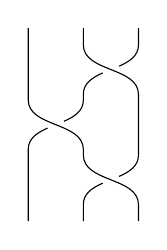
\begin{tikzpicture}[scale=0.7, baseline = -15mm]
	\braid[number of strands = 3] s_2 s_1 s_2;
\end{tikzpicture}
\, = \,
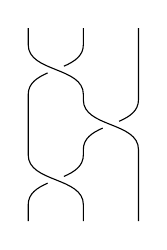
\begin{tikzpicture}[scale=0.7, baseline = -15mm]
	\braid[number of strands = 3] s_1 s_2 s_1;
\end{tikzpicture}\, ,
\end{align*}
and this way of seeing it allows for a certain intuitive interpretation.

\bigno But how exactly do we get a unitary representation of $B_n$ in $TL_n$ from perfect 2-tangles now? Fix some $n$, let $(T_i)_{i=1}^{n-1}$ be perfect 2-tangles with
\begin{align*}
T_i \equiv \alpha_i\cdot  \tikz[scale=0.5, baseline=-1mm]{\foreach \x in {0, 0.5} \draw (\x, -0.5) -- (\x, 0.5);}
 \,+\beta_i\cdot \tikz[scale=0.5, baseline=-1mm]{\draw (0, 0.5) arc[start angle=-180, end angle=0, radius=2.5mm]; \draw (0, -0.5) arc[start angle=180, end angle=0, radius=2.5mm];}\,.
\end{align*}
We will now, disregarding the shading, view these as $n$ tangles via the prescription
\begin{align*}
T_i \overset{\cdot}{=} 1_{i-1} \tensor T_i \tensor 1_{n-i-1} =
\tikz[scale=0.5, baseline=-1mm]{ 
	\draw (0,-1.1) -- node[left] {\tiny$i-1$} (0,1.1); 
	\node[draw] (T) at (1,0) {$T_i$};
	\path 
		($(T.north) + (0.2,0)$)	edge ($(T.north) + (0.2,0.5)$)
		($(T.north) + (-0.2,0)$)	edge ($(T.north) + (-0.2,0.5)$)
		($(T.south) + (0.2,0)$)	edge ($(T.south) + (0.2,-0.5)$)
		($(T.south) + (-0.2,0)$)	edge ($(T.south) + (-0.2,-0.5)$);
	\draw (2,-1.1) -- node[right] {\tiny$n-i-1$} (2,1.1); 
	}
\end{align*}
The first property in the definition of the braid group, $T_i T_j = T_j T_i$ for $\lvert i - j \rvert \geq 2$, is obviously true, but what about the Yang-Baxter relation? There seems to be no quick justification, so we will have to do a few calculations. Firstly w.l.o.g.\ set $n=3$, and we thus only look at $T_1$ and $T_2$. Let us make the substitution $\alpha = \alpha_1$, $\beta = \beta_1$, $\gamma = \alpha_2$, and $\delta = \beta_2$.

The Yang-Baxter equation is now
\begin{align}\label{eq:YB with tangles}
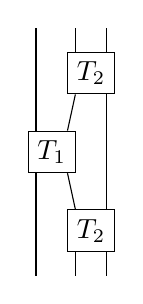
\begin{tikzpicture}[baseline = -2mm]
	\node[draw] (T1) at (0,0) {$T_1$};
	\node[draw] (T2O) at (0.5,1) {$T_2$};
	\node[draw] (T2U) at (0.5,-1) {$T_2$};
	\path 
		($(T2O.south) + (-0.2,0)$) edge ($(T1.north) + (0.2,0)$)
		($(T2O.south) + (0.2,0)$) edge ($(T2U.north) + (0.2,0)$)
		($(T2U.north) + (-0.2,0)$) edge ($(T1.south) + (0.2,0)$);
	\foreach \x in {0.2, -0.2} \draw ($(T2O.north) + (\x, 0)$) -- ($(T2O.north) + (\x, 0.3)$);
	\foreach \x in {0.2, -0.2} \draw ($(T2U.south) + (\x, 0)$) -- ($(T2U.south) + (\x, -0.3)$);
	\draw ($(T1.north) + (-0.2,0)$) -- ($(T1 |- T2O.north) + (-0.2, 0.3)$);
	\draw ($(T1.south) + (-0.2,0)$) -- ($(T1 |- T2U.south) + (-0.2, -0.3)$);
\end{tikzpicture}
\, = \,
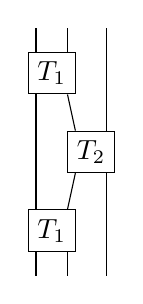
\begin{tikzpicture}[baseline = -2mm]
	\node[draw] (T1) at (0.5,0) {$T_2$};
	\node[draw] (T2O) at (0,1) {$T_1$};
	\node[draw] (T2U) at (0,-1) {$T_1$};
	\path 
		($(T2O.south) + (0.2,0)$) edge ($(T1.north) + (-0.2,0)$)
		($(T2O.south) + (-0.2,0)$) edge ($(T2U.north) + (-0.2,0)$)
		($(T2U.north) + (0.2,0)$) edge ($(T1.south) + (-0.2,0)$);
	\foreach \x in {0.2, -0.2} \draw ($(T2O.north) + (\x, 0)$) -- ($(T2O.north) + (\x, 0.3)$);
	\foreach \x in {0.2, -0.2} \draw ($(T2U.south) + (\x, 0)$) -- ($(T2U.south) + (\x, -0.3)$);
	\draw ($(T1.north) + (0.2,0)$) -- ($(T1 |- T2O.north) + (0.2, 0.3)$);
	\draw ($(T1.south) + (0.2,0)$) -- ($(T1 |- T2U.south) + (0.2, -0.3)$);
\end{tikzpicture} \, ,
\end{align}
and a direct computation of the left hand side yields
\begin{align*}
\begin{pmatrix}
\alpha\gamma^2 \\
\gamma\delta\beta\\
\gamma\delta\beta\\
2\alpha\gamma\delta + q\alpha\delta^2 + \delta^2 \beta\\
\gamma^2\beta
\end{pmatrix},
\end{align*}
where the basis vectors are ordered like in \textsf{Example \ref{ex:TL3}}.

Looking closely, we see that to obtain the right hand side we would have to do the exchanges $\alpha \leftrightarrow \gamma$, $\beta\leftrightarrow\delta$, as well as switching the fourth and fifth entry of the vector. 

We subtract the right hand side from the left hand side and get a total of five equations to be satisfied, namely
\begin{align*}
\begin{pmatrix}
\alpha\gamma^2  - \gamma \alpha^2\\
\gamma\delta\beta - \alpha\beta\delta \\
\gamma\delta\beta - \alpha\beta\delta \\
2\alpha\gamma\delta + q\alpha\delta^2 + \delta^2 \beta - \alpha^2\delta\\
\gamma^2\beta - 2\gamma\alpha\beta - q\gamma\beta^2 - \beta^2 \delta
\end{pmatrix} 
=
0.
\end{align*}
Since all of the four numbers are unequal to zero, the first equation already tells us $\alpha = \gamma$, whence the next two equations follow. Substituting $\alpha$ for $\gamma$ in the last two equations leaves us with
\begin{align*}
\begin{pmatrix}
\alpha^2\delta + q\alpha\delta^2 + \delta^2 \beta \\
\alpha^2\beta +q\alpha\beta^2 +\beta^2 \delta
\end{pmatrix}
=0,
\end{align*}
we can then divide the first of these by $\delta$, the second by $\beta$, obtaining
\begin{align*}
\begin{pmatrix}
\alpha^2 + q\alpha\delta + \delta \beta \\
\alpha^2 +q\alpha\beta+\beta \delta
\end{pmatrix}
=0.
\end{align*}
But now subtract one from the other, and we get $q\alpha(\beta - \delta) \overset{!}{=}0$, hence $\beta = \delta$. So all in all, $T_1 = T_2$. That is, we can only find the braid group within this construction if we build all braidings from the same perfect tangle.

This unitary representation of the braid group\footnote{It is unitary in the sense that if the generator gets mapped to the 2-tangle $T$, then its inverse will be mapped to $T^*$. Of course, this is only a proper representation if we either don't care about multiplicative factors, or if we assume $TT^*=\mathbf{1}_2$. In our setting we don't lose too much sleep over multiplicative factors: In Temperley-Lieb we can always normalize so that $TT^* = \mathbf{1}_2$.}
enables us to apply braidlike operations to construct larger perfect tangles. The first of these procedures, which we will present in the next section, was suggested by Jones and proved by the author. The basic idea is interpreting a perfect 2-tangle $T$ as a braid, which means that multiplying $T$ with its adjoint (which is the horizontally mirrored braid) is really like `\emph{pulling the strings straight, so that there are two parallel strings}'.

%%\documentclass[11pt,a4paper]{article}
%\usepackage[utf8]{inputenc}
%\usepackage[english]{babel}
%\usepackage{amsmath, ifthen,caption}
%\usepackage{amsfonts, amssymb,amsthm, thmtools}
%\usepackage{tikz}\usetikzlibrary{arrows, calc,decorations.markings,cd}
%\usepackage[left=3.5cm,right=3.5cm,top=2.5cm,bottom=4cm]{geometry}
%\declaretheorem[style=definition,qed=$\triangle$]{definition}
%%\declaretheorem[style=definition,qed=$\triangle$,numberwithin=section]{definition}
%\declaretheorem[style=remark,qed=$\blacktriangle$,sibling=definition]{remark}
%\declaretheorem[style=plain,sibling=definition]{theorem}
%\declaretheorem[style=plain,sibling=definition]{lemma}
%\declaretheorem[style=plain,sibling=definition]{proposition}
%\declaretheorem[style=plain,sibling=definition]{example}
%
%\newcommand{\mathbf{1}}{\mathrm{id}}
%
%\title{Constructing arbitrarily large perfect tangles from bi\-unitaries}
%\date{}
%\author{Johannes Berger}
%\begin{document}\maketitle
\section{Constructing Large Perfect Tangles}\label{sec:FirstGeneralConstruction}
First a quick informal discussion to sharpen the intuition. Consider the following braid.
\begin{align*}
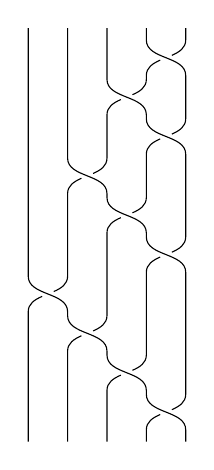
\begin{tikzpicture}[scale = 0.5]
\braid[number of strands = 5] s_4 s_3 s_4 s_2 s_3 s_4 s_1 s_2 s_3 s_4;
\end{tikzpicture}
\end{align*}
Let us try to explain what is happening here: We see that the string starting at position $i$ on the top is attached to position $5-i$ at the bottom. The first rotation will bring the string attached to the left-most point on the top down, and the one attached to the right-most point on the bottom up. But in this setting this is one and the same string! Multiplying with the adjoint of this rotated version will therefore not hinder our efforts in pulling all strings straight. 

Clearly, all subsequent rotations have similar effects. This realization leads to a somewhat educated guess: 
\begin{center}
Tangles built this way are perfect.
\end{center}
The goal of this section is to give both a well-defined construction and a rigorous proof of the statement.

\bigno
To this end, fix a perfect 2-tangle $T\in P_{2\cdot 2}$, and as before things are unshaded.

\begin{definition}\label{def:T}
Let $\widetilde{T}_2\equiv T$, and define inductively for all $n\geq 3$
\begin{align*}
\widetilde{T}_n \equiv\quad
	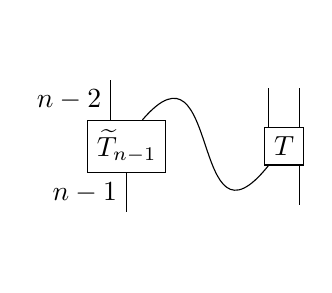
\begin{tikzpicture}[baseline=-0.5mm]
		\node[draw] (T1) at (0,0) {$\widetilde{T}_{n-1}$};
		\node[draw] (T2) at (2,0) {$T$};
%		
		\path ($(T1.north) + (-0.2,0)$) edge node[left]{$n-2$} ($(T1.north) + (-0.2,0.5)$)
			($(T1.south)$) edge node[left]{$n-1$} ($(T1.south) + (0,-0.5)$)
			($(T2.north) + (-0.2,0)$) edge ($(T2.north) + (-0.2,0.5)$)
			($(T2.north) + (0.2,0)$) edge ($(T2.north) + (0.2,0.5)$)
			($(T2.south) + (0.2,0)$) edge ($(T2.south) + (0.2,-0.5)$);		
		\draw  ($(T1.north) + (0.2,0)$) .. controls (1.2,1.5) and (0.8,-1.5).. ($(T2.south) + (-0.2,0)$);
	\end{tikzpicture}\quad .
\end{align*}

Also, with $\widehat{T}_2 \equiv T$, we define the flipped version of this:
\begin{align*}
\widehat{T}_n \equiv\quad
	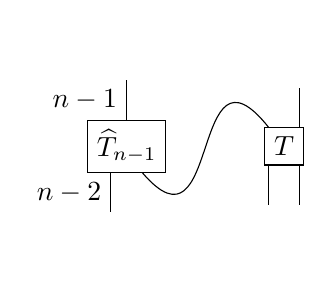
\begin{tikzpicture}[baseline=-0.5mm]
		\node[draw] (T1) at (0,0) {$\widehat{T}_{n-1}$};
		\node[draw] (T2) at (2,0) {$T$};
		\path ($(T1.south) + (-0.2,0)$) edge node[left]{$n-2$} ($(T1.south) + (-0.2,-0.5)$)
			($(T1.north)$) edge node[left]{$n-1$} ($(T1.north) + (0,0.5)$)
			($(T2.south) + (-0.2,0)$) edge ($(T2.south) + (-0.2,-0.5)$)
			($(T2.south) + (0.2,0)$) edge ($(T2.south) + (0.2,-0.5)$)
			($(T2.north) + (0.2,0)$) edge ($(T2.north) + (0.2,0.5)$);		
		\draw  ($(T1.south) + (0.2,0)$) .. controls (1.2,-1.5) and (0.8,1.5).. ($(T2.north) + (-0.2,0)$);
	\end{tikzpicture}\quad,
\end{align*}
which is basically the adjoint of the underlying tangle of $\widetilde{T}_n$, with $T$ inserted into all boxes. Both of these are elements in $P_{2n}$.
\end{definition}

\begin{lemma}\label{lem:T=1}
$\widetilde{T}_n \cdot \widetilde{T}_n^* \propto \mathbf{1}_n$, and a similar result holds for $\widehat{T}_n$.
\begin{proof}
By induction. The base case $n=2$ is clear, since $T$ is perfect. Then suppose that it is true for $n\geq 2$. We get
\begin{align*}
	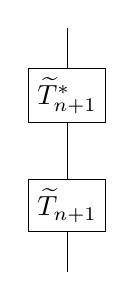
\begin{tikzpicture}[baseline=-1mm]
		\node[draw] (T1) at (0,0.7) {$\widetilde{T}_{n+1}^*$};
		\node[draw] (T2) at (0,-0.7) {$\widetilde{T}_{n+1}$};
		\path
			(T1.north) edge ($(T1.north) + (0,0.5)$)
			(T2.south) edge ($(T2.south) + (0,-.5)$)
			(T1.south) edge (T2.north);
	\end{tikzpicture}
\,&=
	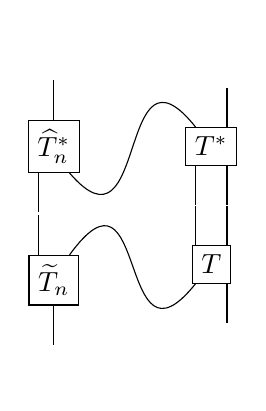
\begin{tikzpicture}[baseline =-8mm]
		\begin{scope}
			\node[draw] (T1) at (0,0) {$\widehat{T}_{n}^*$};
			\node[draw] (T2) at (2,0) {$T^*$};
			\path ($(T1.south) + (-0.2,0)$) edge ($(T1.south) + (-0.2,-0.5)$)
				($(T1.north)$) edge ($(T1.north) + (0,0.5)$)
				($(T2.south) + (-0.2,0)$) edge ($(T2.south) + (-0.2,-0.5)$)
				($(T2.south) + (0.2,0)$) edge ($(T2.south) + (0.2,-0.5)$)
				($(T2.north) + (0.2,0)$) edge ($(T2.north) + (0.2,0.5)$);		
			\draw  ($(T1.south) + (0.2,0)$) .. controls (1.2,-1.5) and (0.8,1.5).. ($(T2.north) + (-0.2,0)$);
		\end{scope}
		\begin{scope}
			\node[draw] (T1) at (0,-1.7) {$\widetilde{T}_{n}$};
			\node[draw] (T2) at (2,-1.5) {$T$};
			\path ($(T1.north) + (-0.2,0)$) edge ($(T1.north) + (-0.2,0.5)$)
				($(T1.south)$) edge ($(T1.south) + (0,-0.5)$)
				($(T2.north) + (-0.2,0)$) edge ($(T2.north) + (-0.2,0.5)$)
				($(T2.north) + (0.2,0)$) edge ($(T2.north) + (0.2,0.5)$)
				($(T2.south) + (0.2,0)$) edge ($(T2.south) + (0.2,-0.5)$);		
			\draw  ($(T1.north) + (0.2,0)$) .. controls (1.2,0) and (0.8,-3).. ($(T2.south) + (-0.2,0)$);
		\end{scope}
	\end{tikzpicture}
\,\propto
	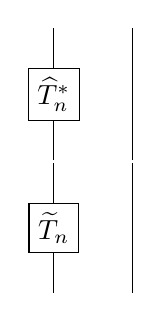
\begin{tikzpicture}[baseline =-8mm]
		\begin{scope}
			\node[draw] (T1) at (0,0) {$\widehat{T}_{n}^*$};
			\path ($(T1.south) + (0,0)$) edge ($(T1.south) + (0,-0.5)$)
				($(T1.north)$) edge ($(T1.north) + (0,0.5)$)
				($(T1.north) + (1,0.5)$) edge ($(T1.south) + (1,-0.5)$);
		\end{scope}
		\begin{scope}
			\node[draw] (T1) at (0,-1.7) {$\widetilde{T}_{n}$};
			\path ($(T1.north) + (0,0)$) edge ($(T1.north) + (0,0.5)$)
				($(T1.south)$) edge ($(T1.south) + (0,-0.5)$)
				($(T1.north) + (1,0.5)$) edge ($(T1.south) + (1,-0.5)$);
		\end{scope}
	\end{tikzpicture}
\, \stackrel{\mathrm{I.H.}}{\propto} \mathbf{1}_{n+1}
\end{align*}
\end{proof}
\end{lemma}

Also note the following:
\begin{equation}\label{eq:concatenation of T}
\begin{tikzpicture}[baseline=-0.5mm]
	\node[draw] (T1) at (0,0) {$\widetilde{T}_{n}$};
	\node[draw] (T2) at (2,0) {$\widetilde{T}_m$};
%
	\path ($(T1.north) + (-.2,0)$) edge ($(T1.north) + (-0.2,0.5)$)
		($(T1.south)$) edge ($(T1.south) + (0,-0.5)$)
		($(T2.north) + (0,0)$) edge ($(T2.north) + (0,0.5)$)
		($(T2.south) + (0.2,0)$) edge ($(T2.south) + (0.2,-0.5)$);		
	\draw  ($(T1.north) + (0.2,0)$) .. controls (1.2,1.5) and (0.8,-1.5).. ($(T2.south) + (-0.2,0)$);
	\node (eq) at (3.5,0) {$= \widetilde{T}_{n+m-1}$};
\end{tikzpicture}
\end{equation}
(here we are contracting a single strand) and similarly for $\widehat{T}_n$, for all $n,m \geq 2$. 

Consider now the following construction:
\begin{definition}\label{def:B}
Let $A_2 \equiv T = \widetilde{T}_2$, and define for $n\geq 3$
\begin{align*}
A_n \equiv \quad
	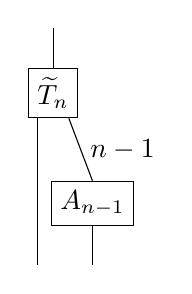
\begin{tikzpicture}[baseline = -1mm]
		\node[draw] (T) at (0,0.7) {$\widetilde{T}_{n}$};
		\node[draw] (B) at (0.5, -.7) {$A_{n-1}$};
		\path (T.north) edge ($(T.north) + (0,0.5)$) 
			($(T.south) + (-0.2, 0)$) edge ($(T.south |- B.south) + (-0.2, -0.5)$)
			($(T.south) + (0.2,0)$) edge node[right]{$n-1$} (B.north)
			($(B.south)$) edge ($(B.south |- B.south) + (-0.0, -0.5)$);
	\end{tikzpicture}\quad .
\end{align*}
\end{definition}

Our goal is to show that each $A_n\in P_{2n}$ is perfect. From \textsf{Lemma \ref{lem:T=1}} it is clear that $A_n \cdot A_n^* \propto \mathbf{1}_n$. This is because \text{Lemma \ref{lem:T=1}} asserts that $\widetilde{T}$s occurring together with their adjoints give (something proportional to) identities until only one box is left (and some strings going straight from the top to the bottom), namely $A_2 = T$. But $T$ is perfect, so this gives (something proportional to) the identity.

\bigskip\noindent A basic yet important and beautiful property of the $A_n$ is now stated.
\begin{lemma}\label{lem:Bcommuting}
For all $n\geq 3$
\begin{align*}
	A_n = \quad
	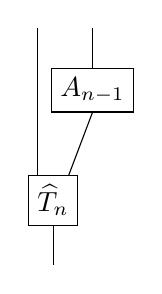
\begin{tikzpicture}[baseline = -1mm]
		\node[draw] (T) at (0,-.7) {$\widehat{T}_{n}$};
		\node[draw] (B) at (0.5, .7) {$A_{n-1}$};
		\path (T.south) edge ($(T.south) + (0,-.5)$) 
			($(T.north) + (-0.2, 0)$) edge ($(T.north |- B.north) + (-0.2, 0.5)$)
			($(T.north) + (0.2,0)$) edge (B.south)
			($(B.north)$) edge ($(B.north |- B.north) + (-0.0, 0.5)$);
	\end{tikzpicture}\quad .
\end{align*}
\begin{proof} By induction. For the base case $n=3$, first remember $A_2=\widetilde{T}_2=\widehat{T}_2 = T$. Then
\begin{align*}
A_3 =\,
	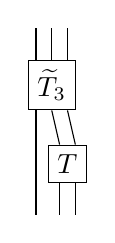
\begin{tikzpicture}[baseline=-2mm]
		\node[draw] (T1) at (0,0.5) {$\widetilde{T}_3$};
		\node[draw] (T2) at (0.2,-0.5) {$T$};
		\foreach \x in {-1,0,1}
			\draw ($(T1.north) + (\x *0.2,0)$) edge ($(T1.north) + (\x *0.2,0.4)$);
		\foreach \x in {-0.1,0.1}{
			\draw ($(T1.south) + (0.1+\x,0)$) -- ($(T2.north) + (\x,0)$);
			\draw ($(T2.south) + (\x,0)$) edge ($(T2.south) + (\x,-0.4)$);
		}
		\draw ($(T1.south) + (-0.2,0)$) edge ($(T1.south |- T2.south) + (-0.2,-0.4)$);
	\end{tikzpicture}
\,&=\,
	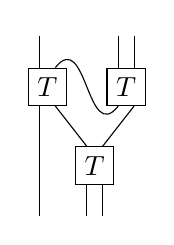
\begin{tikzpicture}[baseline=-2mm]
		\node[draw] (T1) at (0,0.5) {$T$};
		\node[draw] (T2) at (0.6,-0.5) {$T$};
		\node[draw] (T3) at (1,0.5) {$T$};
		\foreach \x in {-0.1,0.1}{
			\draw ($(T3.north) + (\x,0)$) edge ($(T3.north) + (\x,0.4)$);
			\draw ($(T2.south) + (\x,0)$) edge ($(T2.south) + (\x,-0.4)$);
		}
		\draw 
			($(T1.north) + (-0.1,0)$) edge ($(T1.north) + (-0.1,0.4)$)
			($(T1.south) + (-0.1,0)$) edge ($(T1.south |- T2.south) + (-0.1,-0.4)$);
		\path 
			($(T1.south) + (+0.1,0)$) edge ($(T2.north) + (-0.1,0)$)
			($(T3.south) + (+0.1,0)$) edge ($(T2.north) + (0.1,0)$);
		\draw ($(T1.north) + (+0.1,0)$) .. controls ($(T1.north) + (0.5,0.5)$) and ($(T3.south) - (0.5,0.5)$) .. ($(T3.south) + (-0.1,0)$);
	\end{tikzpicture}
\,=\,
	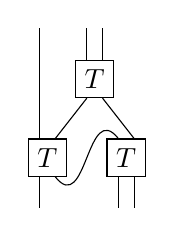
\begin{tikzpicture}[baseline=-2mm]
		\node[draw] (T1) at (0,-0.5) {$T$};
		\node[draw] (T2) at (1,-0.5) {$T$};
		\node[draw] (T3) at (.6,0.5) {$T$};
		\foreach \x in {-0.1,0.1}{
			\draw ($(T3.north) + (\x,0)$) edge ($(T3.north) + (\x,0.4)$);
			\draw ($(T2.south) + (\x,0)$) edge ($(T2.south) + (\x,-0.4)$);
		}
		\draw 
			($(T1.south) + (-0.1,0)$) edge ($(T1.south) + (-0.1,-0.4)$)
			($(T1.north) + (-0.1,0)$) edge ($(T1.north |- T3.north) + (-0.1,0.4)$);
		\path 
			($(T1.north) + (+0.1,0)$) edge ($(T3.south) + (-0.1,0)$)
			($(T3.south) + (+0.1,0)$) edge ($(T2.north) + (0.1,0)$);
		\draw ($(T1.south) + (+0.1,0)$) .. controls ($(T1.south) + (0.5,-0.5)$) and ($(T2.north) - (0.5,-0.5)$) .. ($(T2.north) + (-0.1,0)$);
	\end{tikzpicture}
\,=\,
	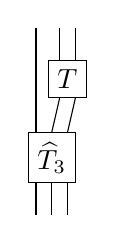
\begin{tikzpicture}[baseline=-2mm]
		\node[draw] (T1) at (0,-0.5) {$\widehat{T}_3$};
		\node[draw] (T2) at (0.2,0.5) {$T$};
		\foreach \x in {-1,0,1}
			\draw ($(T1.south) + (\x *0.2,0)$) edge ($(T1.south) + (\x *0.2,-0.4)$);
		\foreach \x in {-0.1,0.1}{
			\draw ($(T1.north) + (0.1+\x,0)$) -- ($(T2.south) + (\x,0)$);
			\draw ($(T2.north) + (\x,0)$) edge ($(T2.north) + (\x,0.4)$);
		}
		\draw ($(T1.north) + (-0.2,0)$) edge ($(T1.north |- T2.north) + (-0.2,0.4)$);
	\end{tikzpicture}\quad,
\end{align*}
as required. Now suppose that the claim is true up to $n-1$. Then we have
\begin{align*}
A_n &=\,
	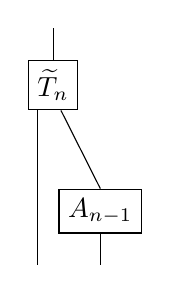
\begin{tikzpicture}[baseline=-2mm]
		\node[draw] (T1) at (0,0.8) {$\widetilde{T}_n$};
		\node[draw] (T2) at (0.6,-0.8) {$A_{n-1}$};
		\draw ($(T1.north) + (0 *0.2,0)$) edge ($(T1.north) + (0 *0.2,0.4)$);
		\draw ($(T1.south) + (0.1+0,0)$) -- ($(T2.north) + (0,0)$);
		\draw ($(T2.south) + (0,0)$) edge ($(T2.south) + (0,-0.4)$);
		\draw ($(T1.south) + (-0.2,0)$) edge ($(T1.south |- T2.south) + (-0.2,-0.4)$);
	\end{tikzpicture}
\,=\,
	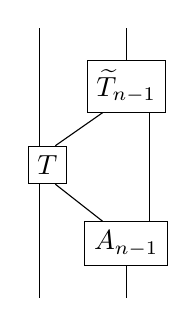
\begin{tikzpicture}[baseline=-2mm]
		\node[draw] (T1) at (0,0) {$T$};
		\node[draw] (Tt) at (1,1) {$\widetilde{T}_{n-1}$};
		\node[draw] (B) at (1,-1) {$A_{n-1}$};
%
		\draw ($(T1.south) + (-0.1,0)$)	edge ($(T1.south |- B.south) + (-0.1,-0.4)$);
		\draw ($(T1.north) + (-0.1,0)$)	edge ($(T1.north |- Tt.north) + (-0.1,0.4)$);
		\path
			($(T1.north) + (0.1,0)$) edge ($(Tt.south) + (-0.3,0)$)
			($(T1.south) + (0.1,0)$) edge ($(B.north) + (-0.3,0)$)
			($(B.north) + (+0.3,0)$)edge ($(Tt.south) + (0.3,0)$);
		\path
			(B.south) edge ($(B.south) + (-0,-0.4)$)
			(Tt.north) edge ($(Tt.north) + (-0,0.4)$);
	\end{tikzpicture}
\,\stackrel{\mathrm{I.H.}}{=}\,
	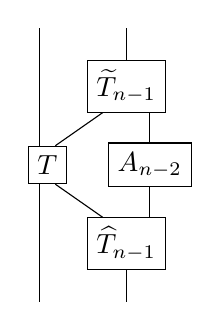
\begin{tikzpicture}[baseline=-2mm]
		\node[draw] (T1) at (0,0) {$T$};
		\node[draw] (Tt) at (1,1) {$\widetilde{T}_{n-1}$};
		\node[draw] (That) at (1,-1) {$\widehat{T}_{n-1}$};
		\node[draw] (B) at (1.3,0) {$A_{n-2}$};
%
		\draw ($(T1.south) + (-0.1,0)$)	edge ($(T1.south |- That.south) + (-0.1,-0.4)$);
		\draw ($(T1.north) + (-0.1,0)$)	edge ($(T1.north |- Tt.north) + (-0.1,0.4)$);
		\path
			($(T1.north) + (0.1,0)$) edge ($(Tt.south) + (-0.3,0)$)
			($(T1.south) + (0.1,0)$) edge ($(That.north) + (-0.3,0)$)
			($(That.north) + (+0.3,0)$)edge ($(B.south) + (0.0,0)$)
			($(B.north) + (+0.0,0)$)edge ($(Tt.south) + (0.3,0)$);
		\path
			(That.south) edge ($(That.south) + (-0,-0.4)$)
			(Tt.north) edge ($(Tt.north) + (-0,0.4)$);
	\end{tikzpicture}\\[1em]
&=\,
	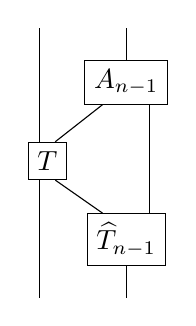
\begin{tikzpicture}[baseline=-2mm]
		\node[draw] (T1) at (0,0) {$T$};
		\node[draw] (Tt) at (1,1) {$A_{n-1}$};
		\node[draw] (B) at (1,-1) {$\widehat{T}_{n-1}$};
%
		\draw ($(T1.south) + (-0.1,0)$)	edge ($(T1.south |- B.south) + (-0.1,-0.4)$);
		\draw ($(T1.north) + (-0.1,0)$)	edge ($(T1.north |- Tt.north) + (-0.1,0.4)$);
		\path
			($(T1.north) + (0.1,0)$) edge ($(Tt.south) + (-0.3,0)$)
			($(T1.south) + (0.1,0)$) edge ($(B.north) + (-0.3,0)$)
			($(B.north) + (+0.3,0)$)edge ($(Tt.south) + (0.3,0)$);
		\path
			(B.south) edge ($(B.south) + (-0,-0.4)$)
			(Tt.north) edge ($(Tt.north) + (-0,0.4)$);
	\end{tikzpicture}
\,=\,
	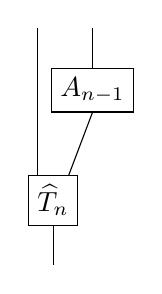
\begin{tikzpicture}[baseline = -2mm]
		\node[draw] (T) at (0,-.7) {$\widehat{T}_{n}$};
		\node[draw] (B) at (0.5, .7) {$A_{n-1}$};
		\path (T.south) edge ($(T.south) + (0,-.5)$) 
			($(T.north) + (-0.2, 0)$) edge ($(T.north |- B.north) + (-0.2, 0.5)$)
			($(T.north) + (0.2,0)$) edge (B.south)
			($(B.north)$) edge ($(B.north |- B.north) + (-0.0, 0.5)$);
	\end{tikzpicture}
\end{align*}
\end{proof}
\end{lemma}

This lemma allows us to switch between two ways of writing $A_n$, which ever way is more comfortable to work with in a given situation. The statement $A_n^*\cdot A_n\propto\mathbf{1}_n$, for example, is now a simple corollary of \textsf{Lemma \ref{lem:Bcommuting}} and the remark made after \textsf{Definition \ref{def:B}}.

One thing we should note is that if we interpret $\widehat{\phantom{T}}_n$ and $\widetilde{\phantom{T}}_n$ as $n$-tangles with $n-1$ internal boxes, then
\begin{align*}
\widetilde{T}_n^* = \widehat{T^*}_n,
\end{align*}
so that $\widetilde{T}_n\cdot \widehat{T^*}_n\propto\mathbf{1}_n$ by \textsf{Lemma \ref{lem:T=1}}.

To prove that the rotations of $A_n$ are also `unitary', we still need to record a few more facts, like the following lemma.
\begin{lemma}\label{lem:half rotated  TT}
Let $1\leq l < n-1$, $n\geq 3$. Then
\begin{align*}
	\begin{tikzpicture}[baseline=-1mm]
			\node[draw] (Tdag) at (0,.7) {$\widetilde{T}_n^*$};
			\node[draw] (T) at (0,-.7) {$\widetilde{T}_n$};
			\path (Tdag.north) edge ($(Tdag.north) + (0,0.5)$)
				(T.south) edge ($(T.south) + (0,-.5)$)
				($(T.north) + (0.2,0)$) edge node[right]{$n-l$} ($(Tdag.south) + (0.2,0)$)
				($(T.north) + (-0.6,0)$) edge node[left] {$l$} ($(T.south) + (-0.6,-0.5)$)
				($(Tdag.south) + (-0.6,0)$) edge node[left] {$l$} ($(Tdag.north) + (-0.6,0.5)$);
			\draw ($(T.north) + (-.2,0)$) arc [start angle=0, end angle=180, radius=0.2cm];
			\draw ($(Tdag.south) + (-.2,0)$) arc [start angle=0, end angle=-180, radius=0.2cm];
	\end{tikzpicture}
\, \propto \,
	\begin{tikzpicture}[baseline=-1mm]
			\node[draw] (Tdag) at (0,.7) {$\widetilde{T}_{l+1}^*$};
			\node[draw] (T) at (0,-.7) {$\widetilde{T}_{l+1}$};
			\path (Tdag.north) edge ($(Tdag.north) + (0,0.5)$)
				(T.south) edge ($(T.south) + (0,-.5)$)
				($(T.north) + (0.2,0)$) edge node[right]{$1$} ($(Tdag.south) + (0.2,0)$)
				($(T.north) + (-0.6,0)$) edge node[left] {$l$} ($(T.south) + (-0.6,-0.5)$)
				($(Tdag.south) + (-0.6,0)$) edge node[left] {$l$} ($(Tdag.north) + (-0.6,0.5)$);
			\draw ($(T.north) + (-.2,0)$) arc [start angle=0, end angle=180, radius=0.2cm];
			\draw ($(Tdag.south) + (-.2,0)$) arc [start angle=0, end angle=-180, radius=0.2cm];
			\draw ($(T.south) + (,-0.5)$) edge node[right]{$n-(l+1)$} ($(Tdag.north) + (1,0.5)$);
	\end{tikzpicture}\,,
\end{align*}
where a string with a 0 next to it is interpreted as no string at all.
\begin{proof}
A computation with careful consideration of the number of strings, and a trick involving \eqref{eq:concatenation of T}, shows the result. We will not write the string count next to each string, so you should definitely do that to help you understand what's going on.

Fix any $n\geq 3$. Here is the calculation:
\begin{align*}
	\begin{tikzpicture}[baseline=-1mm]
			\node[draw] (Tdag) at (0,.7) {$\widetilde{T}_n^*$};
			\node[draw] (T) at (0,-.7) {$\widetilde{T}_n$};
			\path (Tdag.north) edge ($(Tdag.north) + (0,0.5)$)
				(T.south) edge ($(T.south) + (0,-.5)$)
				($(T.north) + (0.2,0)$) edge node[right]{$n-l$} ($(Tdag.south) + (0.2,0)$)
				($(T.north) + (-0.6,0)$) edge node[left] {$l$} ($(T.south) + (-0.6,-0.5)$)
				($(Tdag.south) + (-0.6,0)$) edge node[left] {$l$} ($(Tdag.north) + (-0.6,0.5)$);
			\draw ($(T.north) + (-.2,0)$) arc [start angle=0, end angle=180, radius=0.2cm];
			\draw ($(Tdag.south) + (-.2,0)$) arc [start angle=0, end angle=-180, radius=0.2cm];
	\end{tikzpicture}
\, &= \,
	\begin{tikzpicture}[baseline=-1mm]
		\coordinate (yValue) at (0,1);
		\coordinate (xValue) at (0.7,0);
		\node[draw] (LD) at ($(yValue)-(xValue)$) {$\widetilde{T}_{l+1}^*$};
		\node[draw] (ND) at ($(yValue)+(xValue)$) {$\widetilde{T}_{n-l}^*$};
		\node[draw] (L) at ($(0,0)-(xValue)-(yValue)$) {$\widetilde{T}_{l+1}$};
		\node[draw] (N) at ($(xValue)-(yValue)$) {$\widetilde{T}_{n-l}$};
%
		\coordinate (yMin) at ($(L.south) + (0,-0.4)$);
		\coordinate (yMax) at ($(LD.north) + (0,0.4)$);
		\foreach \x in {-0.3 -0.4, 0.3}
			\draw ($(L.north) + (\x,0)$) arc[start angle=180, end angle=0, radius=2mm];
		\draw ($(LD.south) + (0.3+0.4,0)$) -- ($(ND.north) + (-0.3-0.4,0)$) arc[start angle=180, end angle=0, radius=2mm];
		\foreach \x in {-0.3 -0.4, 0.3}
			\draw ($(LD.south) + (\x,0)$) arc[start angle=-180, end angle=0, radius=2mm];
		\draw ($(L.north) + (0.3+0.4,0)$) -- ($(N.south) + (-0.3-0.4,0)$) arc[start angle=-180, end angle=0, radius=2mm];
		\foreach \x in {LD.north, ND.north}
			\draw (\x) -- (\x |- yMax);
		\draw ($(LD.south)+(-0.3-0.4,0)$) -- ($(LD.south |- yMax)+(-0.3-0.4,0)$);
		\foreach \x in {L.south, N.south}
			\draw (\x) -- (\x |- yMin);
		\draw ($(L.north)+(-0.3-0.4,0)$) -- ($(L.north |- yMin)+(-0.3-0.4,0)$);
		\draw (ND.south) -- (N.north);
	\end{tikzpicture}
\, \propto \,
	\begin{tikzpicture}[baseline=-1mm]
		\coordinate (yValue) at (0,1);
		\coordinate (xValue) at (0.7,0);
		\node[draw] (LD) at ($(yValue)-(xValue)$) {$\widetilde{T}_{l+1}^*$};
		\node[draw] (L) at ($(0,0)-(xValue)-(yValue)$) {$\widetilde{T}_{l+1}$};
%
		\coordinate (yMin) at ($(L.south) + (0,-0.4)$);
		\coordinate (yMax) at ($(LD.north) + (0,0.4)$);
		\foreach \x in {-0.3 -0.4}
			\draw ($(L.north) + (\x,0)$) arc[start angle=180, end angle=0, radius=2mm];
		\foreach \x in {-0.3 -0.4}
			\draw ($(LD.south) + (\x,0)$) arc[start angle=-180, end angle=0, radius=2mm];
		\foreach \x in {LD.north}
			\draw (\x) -- (\x |- yMax);
		\draw ($(LD.south)+(-0.3-0.4,0)$) -- ($(LD.south |- yMax)+(-0.3-0.4,0)$);
		\foreach \x in {L.south}
			\draw (\x) -- (\x |- yMin);
		\draw ($(L.north)+(-0.3-0.4,0)$) -- ($(L.north |- yMin)+(-0.3-0.4,0)$);
		\draw ($(LD.south)+(0.3,0)$) -- ($(L.north)+(0.3,0)$);
		\draw ($(yMin) + (1.2,0)$) -- node[right]{$n-l-1$} ($(yMax) + (1.2,0)$);
	\end{tikzpicture}
\end{align*}
The first equality is the trick, the second (well, not equality but proportionality) uses \textsf{Lemma \ref{lem:T=1}}.
\end{proof}
\end{lemma}

If you read the previous lemma carefully you will probably have noticed that we excluded the $l=n-1$ case. One reason for this is that we can postpone that part until we are in our main theorem, where we solve it by invoking \textsf{Lemma \ref{lem:Bcommuting}}. The other reason is that the formula would be ill-defined, since $n-(n-1) = 1$, but $\widetilde{T}_1$ is undefined.


The following proposition is straightforward, but the result is very useful in one of the last steps in the proof of the main theorem.
\begin{proposition}\label{prop:T rotated n-1 times}
For all $n\geq 2$
\begin{align*}
	\rot^{n-1}\widetilde{T}_n\cdot \left(\rot^{n-1}\widetilde{T}_n\right)^* = 
	\begin{tikzpicture}[baseline=-1mm]
			\node[draw] (Tdag) at (0,.7) {$\widetilde{T}_n^*$};
			\node[draw] (T) at (0,-.7) {$\widetilde{T}_n$};
			\path
				($(Tdag.north) + (-0.2,0)$) edge ($(Tdag.north) + (-0.2,0.5)$)
				($(T.south) + (-0.2,0)$) edge ($(T.south) + (-0.2,-0.5)$)
				($(T.north) + (0.2,0)$) edge ($(Tdag.south) + (0.2,0)$)
				($(T.north) + (-0.6,0)$) edge node[left] {$n-1$} ($(T.south) + (-0.6,-0.5)$)
				($(Tdag.south) + (-0.6,0)$) edge node[left] {$n-1$} ($(Tdag.north) + (-0.6,0.5)$);
			\draw ($(T.north) + (-.2,0)$) arc [start angle=0, end angle=180, radius=0.2cm];
			\draw ($(T.south) + (.2,0)$) arc [start angle=-180, end angle=0, radius=0.2cm] -- node[right]{$n-1$}
				 ($(Tdag.north) + (.6,0)$) arc [start angle=0, end angle=180, radius=0.2cm];
			\draw ($(Tdag.south) + (-.2,0)$) arc [start angle=0, end angle=-180, radius=0.2cm];
	\end{tikzpicture}
\, \propto \mathbf{1}_n
\end{align*}
\end{proposition}
\begin{proof}Omitted. An exercise in mathematical induction for the reader.
\end{proof}

We are now ready to prove our main result.
\begin{theorem}\label{thm:general_existence}
For all $A_n$ the following are true.
\begin{itemize}
	\item[\emph{\text{(i)}}] For all $1\leq l < n$ we have
		\begin{align*}
		\mathrm{rot}^l A_n \cdot \mathrm{rot}^{-l} A_n^* \propto \mathbf{1}_n.
		\end{align*}
	\item[\emph{\text{(ii)}}] $A_n$ is perfect.
\end{itemize}
\begin{proof}
We will first show (i), then (i)$\implies$(ii). The second part is straigthforward.

For (i), first note that this is trivially true for $A_2$, and that proving it for $A_3$ is a basic computation. The base case is thus covered. Now suppose it is true for $n-1$, and consider first $l< n-1$. Then
\begin{align*}
\mathrm{rot}^l A_n \cdot \mathrm{rot}^{-l} A_n^*
&=\,
	\begin{tikzpicture}[baseline=-1mm]
		\node[draw] (BD) at (1,2) {$A_{n-1}^*$};
		\node[draw] (TD) at (0,0.8) {$\widetilde{T}_n^*$};
		\node[draw] (T) at (0,-0.8) {$\widetilde{T}_n$};
		\node[draw] (B) at (1, -2) {$A_{n-1}$};
		\coordinate (yMax) at ($(BD.north)+(0,0.4)$);
		\coordinate (yMin) at ($(B.south)+(0,-0.4)$);
		\draw 
			($(B.south)+(0.4,0)$) arc[start angle=-180, end angle=0, radius=2mm] -- node[right] {$l$}
			($(BD.north)+(0.8,0)$) arc[start angle=0, end angle=180, radius=2mm];
		\path 
			($(TD.north)+(0.2,0)$) edge ($(BD.south)+(-0.4,0)$)
			($(TD.south)+(0.2,0)$) edgenode[right] {$n-l$}  ($(T.north)+(0.2,0)$)
			($(T.south)+(0.2,0)$) edge ($(B.north)+(-0.4,0)$);
		\draw
			($(TD.south)+(-0.2,0)$) arc[start angle=0, end angle=-180, radius=2mm] edge node[left] {$l$} ($(TD.south |- yMax)+(-0.6,0)$);
		\draw
			($(T.north)+(-0.2,0)$) arc[start angle=0, end angle=180, radius=2mm] edge node[left] {$l$} ($(TD.south |- yMin)+(-0.6,0)$);
		\path
			($(BD.north)+(-0.2,0)$) edge ($(BD.north |- yMax)+(-0.2,0)$)
			($(TD.north)+(-0.2,0)$) edge ($(TD.north |- yMax)+(-0.2,0)$)
			($(T.south)+(-0.2,0)$) edge ($(T.south |- yMin)+(-0.2,0)$)
			($(B.south)+(-0.2,0)$) edge ($(B.south |- yMin)+(-0.2,0)$);
	\end{tikzpicture}
\,=\,
	\begin{tikzpicture}[baseline=-1mm]
		\node[draw] (BD) at (1,2) {$A_{n-1}^*$};
		\node[draw] (TD) at (0,0.8) {$\widetilde{T}_{l+1}^*$};
		\node[draw] (T) at (0,-0.8) {$\widetilde{T}_{l+1}$};
		\node[draw] (B) at (1, -2) {$A_{n-1}$};
		\coordinate (yMax) at ($(BD.north)+(0,0.4)$);
		\coordinate (yMin) at ($(B.south)+(0,-0.4)$);
		\draw 
			($(B.south)+(0.4,0)$) arc[start angle=-180, end angle=0, radius=2mm] -- node[right] {$l$}
			($(BD.north)+(0.8,0)$) arc[start angle=0, end angle=180, radius=2mm];
		\path 
			($(TD.north)+(0.2,0)$) edge node[right]{$l$} ($(BD.south)+(-0.4,0)$)
			($(TD.south)+(0.2,0)$) edge node[right] {$1$}  ($(T.north)+(0.2,0)$)
			($(T.south)+(0.2,0)$) edge ($(B.north)+(-0.4,0)$);
		\draw
			($(BD.south)+(+0.4,0)$) edge node[above, rotate=90]{{\small$n-1-l$}}  ($(B.north)+(0.4,0)$);
		\draw
			($(TD.south)+(-0.2,0)$) arc[start angle=0, end angle=-180, radius=2mm] edge node[left] {$l$} ($(TD.south |- yMax)+(-0.6,0)$);
		\draw
			($(T.north)+(-0.2,0)$) arc[start angle=0, end angle=180, radius=2mm] edge node[left] {$l$} ($(TD.south |- yMin)+(-0.6,0)$);
		\path
			($(BD.north)+(-0.2,0)$) edge ($(BD.north |- yMax)+(-0.2,0)$)
			($(TD.north)+(-0.2,0)$) edge ($(TD.north |- yMax)+(-0.2,0)$)
			($(T.south)+(-0.2,0)$) edge ($(T.south |- yMin)+(-0.2,0)$)
			($(B.south)+(-0.2,0)$) edge ($(B.south |- yMin)+(-0.2,0)$);
	\end{tikzpicture}\\[2em]
\, &\propto \,
	\begin{tikzpicture}[baseline=-1mm]
			\node[draw] (Tdag) at (0,.7) {$\widetilde{T}_{l+1}^*$};
			\node[draw] (T) at (0,-.7) {$\widetilde{T}_{l+1}$};
			\path
				($(Tdag.north) + (-0.2,0)$) edge ($(Tdag.north) + (-0.2,0.5)$)
				($(T.south) + (-0.2,0)$) edge ($(T.south) + (-0.2,-0.5)$)
				($(T.north) + (0.2,0)$) edge ($(Tdag.south) + (0.2,0)$)
				($(T.north) + (-0.6,0)$) edge node[left] {$l$} ($(T.south) + (-0.6,-0.5)$)
				($(Tdag.south) + (-0.6,0)$) edge node[left] {$l$} ($(Tdag.north) + (-0.6,0.5)$);
			\draw ($(Tdag.north) + (1.5,0.5)$) -- node[right]{$n-1-l$} ($(T.south) + (1.5,-0.5)$);
%			
			\draw ($(T.north) + (-.2,0)$) arc [start angle=0, end angle=180, radius=0.2cm];
			\draw ($(T.south) + (.2,0)$) arc [start angle=-180, end angle=0, radius=0.2cm] -- node[right]{$l$}
				 ($(Tdag.north) + (.6,0)$) arc [start angle=0, end angle=180, radius=0.2cm];
			\draw ($(Tdag.south) + (-.2,0)$) arc [start angle=0, end angle=-180, radius=0.2cm];
	\end{tikzpicture}\\[2em]
&\propto \mathbf{1}_n
\end{align*}
What's happening here is the following. The first step is writing out the definition. The second is applying \textsf{Lemma \ref{lem:half rotated  TT}}, after which we are at the induction step: it's true that $\mathrm{rot}^l A_{n-1} \cdot \mathrm{rot}^{-l} A_{n-1}^* \propto \mathbf{1}_{n-1}$. Note that the largest value of $l$ here is $(n-1)-1$.
Last but not least, we invoke \textsf{Proposition \ref{prop:T rotated n-1 times}}, which gives the desired result.

For $l=n-1$ note that the rotation bends \emph{all} legs of $A_{n-1}$ up- and all legs of $A_{n-1}^*$ downwards, thereby contracting the $A$s along half of their legs. That is we have the product $A_{n-1}^*\cdot  A_{n-1}$, which, as we have argued before, is proportional to $\mathbf{1}_{n-1}$. Then all that's left is applying \textsf{Proposition \ref{prop:T rotated n-1 times}} one time and the proof of part (i) is finished.

\bigskip
Part (ii) of the theorem follows from \textsf{Proposition \ref{Prop:ROT INVROT}}, i.e.\
\begin{align*}
0\leq l <k : \mathrm{rot}^{k+l} T\cdot\mathrm{rot}^{-(k+l)}T^* \propto \mathbf{1}_k \quad\iff\quad \mathrm{rot}^{-l}T^* \cdot \mathrm{rot}^{l} T\propto \mathbf{1}_k,
\end{align*}
and an argument about the validity of `horizontally flipped' versions of \textsf{Lemma \ref{lem:half rotated  TT}} and \textsf{Proposition \ref{prop:T rotated n-1 times}}, after seeing that the base case is (almost trivially) true.\footnote{In the TL planar algebra, one could also make a handwavy argument that actually follows from $\rot^n A_n = A_n$, like so. Observe that $T\in TL_2$ is necessarily symmetric under rotation by 2 clicks. Then we have $\rot^n\widetilde{T}_n = \widetilde{T}_n$, and consequently the same holds for $A_n$ because it's made up of $\widetilde{T}$s.} 
%about the symmetry of $A_n$ shown in Lemma \ref{lem:Bcommuting}, as well as interpreting $\widetilde{\phantom{T}}_n$ as a tangle with $n-1$ internal boxes.
\end{proof}
\end{theorem}

These perfect tangles constructed in this section are certainly very pretty. In \figref{fig:examples_general_construction} we see a few examples which are in $P_{2n}$ for $n=3,4,5,6$, respectively. The perfect tangle $T\in TL_{2\cdot 2}$ is represented as a vertex and should be interpreted as being in standard form [\emph{cf.\ the very second page of this thesis}].
\begin{figure}[!htp]\centering
\captionsetup{width=.7\linewidth}
\begin{tikzpicture}[inner sep=0.5mm,scale=1]
	\foreach \order in {1,...,4}{
		\begin{scope}[xshift=1/2*\order*\order cm]
			\coordinate (yMax) at (0, .7+ 0.5*\order);
			\coordinate (yMin) at (0,-.7-.5*\order);
			\foreach \x in {0,...,\order}{
				\foreach \y in {0,...,\x}{		
					\node[draw, fill,circle] (x\x) at (.8*\x,.5*\x -1*\y) {};
					\ifthenelse{\NOT \x = \order}{
						\draw (x\x) -- ($(x\x) + (.8, .5 - 1)$);
						\draw (x\x) -- ($(x\x) + (.8, -.5 + 1)$);
						\ifthenelse{\y=\x}{
							\ifthenelse{\y=0}{\draw (x\x) -- (x\x |- yMax);}{}
							\draw (x\x) -- (x\x |- yMin);}{\ifthenelse{\y=0}{\draw (x\x) -- (x\x |- yMax);}{}
						}
					}{
						\ifthenelse{\y=0}{
							\draw (x\x) -- ($(x\x) + (0,-\order)$);
							\draw ($(x\x.north) + (0.05,-0.05)$) -- ($(x\x.north |- yMax) + (0.05, 0)$);
							\draw ($(x\x.north) - (0.05, 0.05)$) -- ($(x\x.north |- yMax) - (0.05,0)$);
						}{
							\ifthenelse{\y=\x}{
							\draw ($(x\x.south) - (0.05,-0.05)$) -- ($(x\x.south |- yMin) - (0.05, 0)$);
							\draw ($(x\x.south) +(0.05, 0.05)$) -- ($(x\x.south |- yMin) + (0.05,0)$);
							}{}
						}
					}
				}
			}
			\ifthenelse{\NOT \order=4}{\node (comma) at (0.2+.8*\order,0) {$,$};}{}
		\end{scope}
	}
\end{tikzpicture}
\caption[Examples of perfect tangles obtained by the iterative construction proved in \textsf{Theorem \ref{thm:general_existence}}]{The perfect tangles $A_3,A_4,A_5,A_6$. Vertices represent the generating perfect 2-tangle $T$ in standard form.}
\label{fig:examples_general_construction}
\end{figure}


It is clear that what this theorem actually does is that it gives us for each $n$ an $n$-tangle with $\frac{n(n-1)}{2}$ internal 2-boxes, such that if we fix a perfect 2-tangle and insert a copy into each box the resulting element is perfect.

%If we let $P_n$ denote the set of perfect $n$-tangles with
%\begin{align*}
%T\in P_n \quad \implies \quad \rot^l(T) \not \in P_n\qquad \forall 0 < l < 2n,
%\end{align*}

In the next section we will argue (but not show) that this construction, among others, works for any planar algebra with perfect $2$-tangles. Letting $\mathcal{P}_n$ denote the set of perfect $n$-tangles --- including adjoints and rotations of tangles already in $\mathcal{P}_n$ --- then \textsf{Theorem \ref{thm:general_existence}} shows a lower bound on the size of this set:
\begin{align}\label{eq:lower_bound no1}
\lvert \mathcal{P}_2 \rvert \leq \lvert \mathcal{P}_n \rvert \quad \forall n\geq 2.
\end{align}
So whenever $\mathcal{P}_2\neq \emptyset$, the general existence of perfect tangles in spaces indexed by an even color is established.

%\section{Going even further: Raising the lower bound}
%The fact that the procedure of constructing $A_n$ yields an $n$-tangle, together with the observation of how the proof of Theorem \ref{thm:general_existence} actually works, raises some hope of a further generalization --- an even better result. 
%
%The section is devoted to stating \emph{and} proving this more general version, effectively raising the lower bound given in equation (\ref{eq:lower_bound no1}). We will first state it as a (justified) conjecture, which will then, over the course of this section, be proven.
%
%\bigno
%Take the $n$-tangle $A_n$ from the previous section, and `remove' all $T$s.  By the very definition of planar tangles, we are then left with a multilinear map, which we shall denote by
%\begin{align*}
%\widetilde{B}_n:\bigtimes_{i=1}^{\frac{n(n-1)}{2}} TL_2 \rightarrow TL_n.
%\end{align*}
%Because of the high symmetry of $A_n$, and looking back at the proof of the big theorem in the last section, we are led to the following:
%
%
%\begin{center}\boxed{
%	\begin{minipage}{0.85\textwidth}\textbf{\textsf{Educated Hunch.}}\\
%		Using the notation $P_n$ for the set of all perfect tangles, we first claim
%	\begin{align*}\label{conjecture:1}\tag{\textsf{Hunch 1}}
%		\widetilde{B}_n\left( P_2^{\frac{n(n-1)}{2}} \right) \subset P_n,\footnotemark
%	\end{align*}
%	that is any $\frac{n(n-1)}{2}$-tuple of perfect 2-tangles gets mapped to a perfect $n$-tangle.
%
%	\bigno
%	The second claim that we make is: $\widetilde{B}_n$ restricted to perfect 2-tangles is bijective onto its image. That is we allege that the map
%	\begin{align*}\label{conjecture:2} \tag{\textsf{Hunch 2}}
%		\at{\widetilde{B}_n}{P_2^{\frac{n(n-1)}{2}}} : P_2^{\frac{n(n-1)}{2}} \longrightarrow P_n%TL_n
%	\end{align*}
%	is injective, thus effectively raising the lower bound (\ref{eq:lower_bound no1}) on the number of \emph{distinct} perfect $n$-tangles from $\lvert P_2 \rvert$ to
%	\begin{align*}
%		\lvert P_2 \rvert^{\frac{n(n-1)}{2}} \leq \lvert P_n \rvert
%	\end{align*}
%	\end{minipage}
%}\end{center}\footnotetext{If $S$ is a set and $k$ is a natural number, then $S^k$ is the $k$th Cartesian power of $S$.}
%
%\ref{conjecture:1}
%It is important to emphasize that $TL_n\subset \mathcal{C}_{2n}$ (the hom-space $\mathcal{C}[1,X^{\otimes 2n}]$). By construction, any $A_n$ can thus be interpreted as a morphism in a trivalent category, which, in particular, is perfect. So this section not only gave us a ton of perfect tangles, but also more than enough perfect morphism!
%\end{document}


\section{A Conjecture}
Motivated by the results of the previous section we will here state a conjecture which, if true, basically asserts that there is a simple method of of obtaining infinitely many constructions of larger perfect tangles from smaller ones. This conjecture is split into multiple parts and stems from the same observation that gave rise to the construction discussed in the previous section.

As a first example, consider the following tangle:
\begin{align}\label{eq:HorizontalConstruction}
T(\bullet, \bullet) \equiv \,
\begin{tikzpicture}[scale=1.7, baseline=-1mm]
%	\node[draw, blue] (A) at (-0.5,0) {$1$};
%	\node[draw, red] (B) at (0.5,0) {$2$};
%%
%	\draw[blue] ($(A.north) + (0.05,0)$) .. controls +(up:1mm)  .. + (0.8,1);
%	\draw[blue] ($(A.south) + (0.05,0)$) .. controls +(down:1mm)  .. + (0.8,-1);
%	\draw[blue] ($(A.north) + (-0.05,0)$) .. controls +(up:1mm)  ..+ (0.4,1);
%	\draw[blue] ($(A.south) + (-0.05,0)$) .. controls +(down:1mm)  ..+ (0.4,-1);	
%%
%	\draw[red] ($(B.north) + (0.05,0)$) --+ (0,1);
%	\draw[red] ($(B.south) + (0.05,0)$) --+ (0,-1);
%	\draw[line width=4pt,white] ($(B.north) + (-0.05,0)$) .. controls +(up:1mm)  .. ($(A.north) + (-0.05,1)$) ;
%	\draw[red] ($(B.north) + (-0.05,0)$) .. controls +(up:1mm)  .. ($(A.north) + (-0.05,1)$) ;	\
%	\draw[line width=4pt, white] ($(B.south) + (-0.05,-0)$) .. controls +(down:1mm)  .. ($(A.south) + (-0.05,-1)$) ;
%	\draw[red] ($(B.south) + (-0.05,0)$) .. controls +(down:1mm)  .. ($(A.south) + (-0.05,-1)$) ;
%	
	\node[draw, black] (A) at (-0.5,0) {$1$};
	\node[draw, black] (B) at (0.5,0) {$2$};
%
	\draw[black] ($(A.north) + (0.05,0)$) .. controls +(up:1mm)  .. + (0.8,1);
	\draw[black] ($(A.south) + (0.05,0)$) .. controls +(down:1mm)  .. + (0.8,-1);
	\draw[black] ($(A.north) + (-0.05,0)$) .. controls +(up:1mm)  ..+ (0.4,1);
	\draw[black] ($(A.south) + (-0.05,0)$) .. controls +(down:1mm)  ..+ (0.4,-1);	
%
	\draw[black] ($(B.north) + (0.05,0)$) --+ (0,1);
	\draw[black] ($(B.south) + (0.05,0)$) --+ (0,-1);
	\draw[line width=4pt,white] ($(B.north) + (-0.05,0)$) .. controls +(up:1mm)  .. ($(A.north) + (-0.05,1)$) ;
	\draw[black] ($(B.north) + (-0.05,0)$) .. controls +(up:1mm)  .. ($(A.north) + (-0.05,1)$) ;	\
	\draw[line width=4pt, white] ($(B.south) + (-0.05,-0)$) .. controls +(down:1mm)  .. ($(A.south) + (-0.05,-1)$) ;
	\draw[black] ($(B.south) + (-0.05,0)$) .. controls +(down:1mm)  .. ($(A.south) + (-0.05,-1)$) ;
\end{tikzpicture}
\end{align}
We now assume that we insert perfect tangles into both boxes, and without loss call the the resulting tangle $T$. 

Without making any reference to the braid group, i.e.\ without substituting the crossings with perfect tangles, we can still make the argument that $T\cdot T^*\propto \mathbf{1}_4$. This is easily seen by simply pulling the strings straight. Even more so, we can quickly see that this is actually true for all rotations, i.e.\ $\rot^l T \cdot \rot^{-l}T^* \propto \mathbf{1}_4$, by observing that the legs that are bent down and the legs that are bent up `belong' to the same internal box, for each rotation.

Part of the conjecture is now that this yields a sort of \emph{horizontal construction} of perfect tangles, by the following rule.\footnote{Note that this is only for tangles with an even number of legs.}
\begin{conjecture}
From an $n$-tangle $T$ and an $m$-tangle $S$, both perfect, and a fixed perfect $2$-tangle $R$ one can build perfect $(n+m)$-tangles by following a few simple steps:
\begin{itemize}
\item[•] Look at $T\tensor S$, i.e.\ draw the tangles next to each other, as boxes in standard form, so that their respective `midpoints' lie on some imagined $x$-axis.
\item[•] Braid the lower legs in any way you want, but subject to the requirement that strings coming from the same box don't cross. By lower legs we mean all $n+m$ legs in the negative $y$ portion of the plane.
\item[•] Mirror the same braiding for the upper legs. \emph{Mirroring} is here supposed to mean the following, by example: If, counting from the left, the $r$th lower leg of $S$ is braided down to the $l$th position, $1\leq l \leq n+m$, then the $(m-r+1)$th upper leg must be braided to position $n+m-l+1$. This, in a sense, mimics \emph{reflection at a point}.
\item[•] Replace all crossings by $R$.
\end{itemize}
If we call the braiding of the lower legs $\mathcal{L}$, then the tangle obtained via the above procedure shall be denoted by the symbol 
\begin{align*}
T \oslash_\mathcal{L} S
\end{align*}
\end{conjecture}
To be fair, this is pretty confusing, so another example for $n=m=3$, given in \figref{fig:HorizontalConstruction}, should illuminate this. 
\begin{figure}[!htp]\centering
\begin{tikzpicture}[scale=2]
	\node[draw, blue,line width=1pt] (A) at (-1,0) {$\phantom{\hat{ABC}^2}$};
	\node[draw, red,line width=1pt] (B) at (1,0) {$\phantom{\hat{ABC}^2}$};

	\draw[blue,line width=1pt] ($(A.north) - (0.2,0)$) .. controls +(up:1mm)  .. + (0.5, 1);
	\draw[blue,line width=1pt] ($(A.north) - (0,0)$) .. controls +(up:1mm)  .. + (1.2, 1);
	\draw[blue,line width=1pt] ($(A.north) + (0.2,0)$) .. controls +(up:1mm)  .. + (2, 1);
	
	\draw[blue,line width=1pt] ($(A.south) - (0.2,0)$) -- +(0, -1);
	\draw[blue,line width=1pt] ($(A.south) - (0,0)$) .. controls +(down:1mm)  .. +(0.8, -1);
	\draw[blue,line width=1pt] ($(A.south) + (0.2,0)$) .. controls +(down:1mm)  .. +(1.8, -1);
	
	\draw[line width=6pt, white] ($(B.north) + (0.2,0)$) .. controls +(up:1mm)  ..  + (-0.5, 1);
	\draw[line width=6pt, white] ($(B.north) - (0,0)$) .. controls +(up:1mm)  .. + (-1.2, 1);
	\draw[line width=6pt, white] ($(B.north) - (0.2,0)$) .. controls +(up:1mm)  .. + (-2, 1);	
	\draw[red,line width=1pt] ($(B.north) + (0.2,0)$) .. controls +(up:1mm)  .. + (-0.5, 1);
	\draw[red,line width=1pt] ($(B.north) - (0,0)$) .. controls +(up:1mm)  .. + (-1.2, 1);
	\draw[red,line width=1pt] ($(B.north) - (0.2,0)$) .. controls +(up:1mm)  .. + (-2, 1);
	
	\draw[line width=6pt, white] ($(B.south) + (0.2,0)$) -- +(0, -1);
	\draw[line width=6pt, white] ($(B.south) - (0,0)$) .. controls +(down:1mm)  .. +(-0.8, -1);
	\draw[line width=6pt, white] ($(B.south) - (0.2,0)$) .. controls +(down:1mm)  .. +(-1.8, -1);
	\draw[red,line width=1pt] ($(B.south) + (0.2,0)$) -- +(0, -1);
	\draw[red,line width=1pt] ($(B.south) - (0,0)$) .. controls +(down:1mm)  .. +(-0.8, -1);
	\draw[red,line width=1pt] ($(B.south) - (0.2,0)$) .. controls +(down:1mm)  .. +(-1.8, -1);
\end{tikzpicture}
\caption[Horizontal construction of larger perfect tangles]{Obtaining a perfect $6$-tangle from two perfect $3$-tangles via the horizontal construction. On the bottom we braided so that no two strings of the same color are next to another, and with red on the left. Consequently, on the top we need red on the right, and still the colors have to alternate. It is easy, albeit fairly tedious, to verify that this tangle is perfect, given that the 3-boxes and the crossings are perfect.}
\label{fig:HorizontalConstruction}
\end{figure}

It should be noted that we did already prove a special of this conjecture, in the previous section. Fixing any perfect 2-tangle $T$ and with the trivial braidings, we see that if $A_2 = T = \mathbf{1}\oslash_\emptyset \mathbf{1}_1$, then $A_3 = \mathbf{1}_1\oslash_{\mathbf{1}_3} T$, and $A_n = \mathbf{1}_1\oslash_{\mathbf{1}_n} A_{n-1}$.

\begin{conjecture}
Let $T,S$ as in the previous conjecture. Fix a braiding $\mathcal{L}$. 

Then it is not necessary to insert the same perfect $2$-tangle for each braiding, yet the conjecture is still valid. That is, if we enumerate all crossings in $T\oslash_\mathcal{L}S$ --- call the $i$th one $c_i$ --- then in $\rot^l \left(T\oslash_\mathcal{L}S\right) \cdot \rot^{-l}\left( T\oslash_\mathcal{L} S \right)^*$, the crossing $c_i$ in the first factor will always \emph{annihilate} with the obvious crossing $c_i^*$ in the second factor.

In particular this works for any planar algebra where biunitaries exist.
\end{conjecture}
It is clear that this also works when writing multiple perfect tensors next to each other, because then the collection of perfect tangles is closed under $\oslash$. But associativity is, a priori. not satisfied. For example, a quick calculations shows that
\begin{align*}
\left( \mathbf{1}_2\oslash_\mathbf{1}  \mathbf{1}_2  \right) \oslash_ \mathbf{1}  \mathbf{1}_2 =  \mathbf{1}_2 \oslash_ \mathbf{1} \left(  \mathbf{1}_2 \oslash_ \mathbf{1}  \mathbf{1}_2 \right) \implies \text{a `higher Yang-Baxter relation' is satisfied}
\end{align*}
only if a `higher Yang-Baxter relation' is satisfied. This is always the case if perfect $2$-tangles realize the braid group, such as in Temperley-Lieb, but in general it is not satisfied.

\bigno A proof by hand-waving is easy, and the validity of small examples is (more or less) quickly verified. But a \emph{good} proof should be verifiable by a computer program. Thus this remains a conjecture: So far, there is no (obvious) way of writing these constructions inductively so that a proof by induction easily follows.

\bigno To emphasize the actual extent of this:
\begin{center}
\begin{minipage}{0.8\textwidth}
If true, then this also holds for perfect tensors, and by simply fixing a 4-leg perfect tensor (these exist) to substitute the crossings with, we get an incredibly rich family of constructions for larger perfect tensors.
\end{minipage}
\end{center}

\section{Some Explicit Examples}\label{section:EXAMPLES}
In this section we will finally reveal a few of the perfect tangles found via the various means developed during this master's project, i.e.\ one found with computational aid, and those built from smaller ones using the approaches discussed in the previous sections.

\subsection*{Keeping it Simple: \texorpdfstring{$TL_2$}{TL}}\addcontentsline{toc}{subsection}{Keeping it Simple: \texorpdfstring{$TL_2$}{TL}}
Examples here only exist when $0< q \leq 2$, as will become apparent. We have already seen the equations that must be satisfied so that the 2-tangle 
\begin{align*}
T \equiv \alpha\,  \tikz[scale=0.5, baseline=-1mm]{\foreach \x in {0, 0.5} \draw (\x, -0.5) -- (\x, 0.5);}
 \,+\beta\, \tikz[scale=0.5, baseline=-1mm]{\draw (0, 0.5) arc[start angle=-180, end angle=0, radius=2.5mm]; \draw (0, -0.5) arc[start angle=180, end angle=0, radius=2.5mm];}\,,
\end{align*}
is perfect, but let us restate them anyways:
\begin{alignat*}{2}
\lvert \alpha \rvert^2 &\neq 0, \qquad &
\alpha \overline{\beta} + \overline{\alpha}\beta + q\lvert \beta \rvert^2 \overset{!}{=}0, \\
\lvert \beta \rvert^2 &\neq 0,\qquad &
\alpha \overline{\beta} + \overline{\alpha}\beta + q\lvert \alpha \rvert^2 \overset{!}{=}0.
\end{alignat*}

We normalize, i.e.\ $\alpha = 1$, and note that $\lvert \beta \rvert^2 =\lvert \alpha \rvert^2 = 1$. Thus $\beta = e^{i\theta}$. Reinserting this into, say, the second equation we obtain
\begin{align*}
e^{-i\theta} + e^{i\theta}  + q = 0,
\end{align*}
whence
\begin{align*}
\cos(\theta) = -\frac{q}{2}.
\end{align*}
Thus $\theta = \pm \arccos\left(-\frac{q}{2}\right)$, the $\pm$ coming from the cosine being even. This is well-defined since $0<q\leq 2$ by assumption. 

For $n\geq 3$ let
\begin{align*}
f(q)\equiv 
\begin{cases}
\frac{n-1}{n}\pi & \text{if } q=2\cos \frac{\pi}{n} \\
\pi &\text{if } q = 2 \\
\arccos\left( -\frac{q}{2} \right) & \text{else}
\end{cases}.
\end{align*}
The solutions are then given by
\begin{align*}
\alpha = 1, \qquad \beta = e^{\pm i f(q)}=
\begin{cases}
\exp\left( \pm i \frac{n-1}{n} \pi \right) & q = 2\cos \frac{\pi}{n}\\
-1 & q = 2 \\
-\frac{q}{2} \pm \frac{i}{2}\sqrt{4-q^2} & \text{else}
\end{cases}.
\end{align*}

\subsection*{Building Larger Tangles}\addcontentsline{toc}{subsection}{Building Larger Tangles}

We will now use the theorem from \textsf{Section \ref{sec:FirstGeneralConstruction}} to get a perfect tangle in $TL_3$ from one in $TL_2$ . In our discussion of the braid group and $TL_2$ we have seen what the 3-tangle obtained from the construction will look like, namely on the left hand side of \eqref{eq:YB with tangles}.

We already computed that side, and now only need so substitute $\alpha, \gamma$ with 1, and $\beta, \delta$ with $\exp\left(\pm i f(q) \right)$, which yields
\begin{align*}
\begin{tikzpicture}[baseline = -2mm]
	\node[draw] (T1) at (0,0) {$T_\pm$};
	\node[draw] (T2O) at (0.5,1) {$T_\pm$};
	\node[draw] (T2U) at (0.5,-1) {$T_\pm$};
	\path 
		($(T2O.south) + (-0.2,0)$) edge ($(T1.north) + (0.2,0)$)
		($(T2O.south) + (0.2,0)$) edge ($(T2U.north) + (0.2,0)$)
		($(T2U.north) + (-0.2,0)$) edge ($(T1.south) + (0.2,0)$);
	\foreach \x in {0.2, -0.2} \draw ($(T2O.north) + (\x, 0)$) -- ($(T2O.north) + (\x, 0.3)$);
	\foreach \x in {0.2, -0.2} \draw ($(T2U.south) + (\x, 0)$) -- ($(T2U.south) + (\x, -0.3)$);
	\draw ($(T1.north) + (-0.2,0)$) -- ($(T1 |- T2O.north) + (-0.2, 0.3)$);
	\draw ($(T1.south) + (-0.2,0)$) -- ($(T1 |- T2U.south) + (-0.2, -0.3)$);
\end{tikzpicture}
\, &= \,
\begin{pmatrix}
1 \\
\beta^2\\
\beta^2\\
2\beta + q\beta^2 + \beta^3 \\
\beta
\end{pmatrix}\\
&=e^{\pm i f(q)}
\begin{pmatrix}
e^{\mp i f(q)}\\
e^{\pm i f(q)}\\
e^{\pm f(q)}\\
 2 + qe^{\pm i f(q)} + e^{\pm 2i f(q)}\\
1
\end{pmatrix}\\
&=
e^{\pm i f(q)}\left\{
	e^{\mp i f(q)}\,
	\begin{tikzpicture}[scale = 0.7, baseline=-1mm]
		\foreach \x in {-0.5,0,0.5}
			\draw (\x, 0.8) -- (\x,-0.8);
	\end{tikzpicture}
	+ e^{\pm i f(q)}
	\left(\,
		\begin{tikzpicture}[scale = 0.7, baseline=-1mm]
			\draw (0,0.8) .. controls (0,-0.5+0.8) and (0.5,-0.5+0.8) .. (0.5,0.8);
			\draw (-0.5,-0.8) .. controls (-0.5,1-0.5-0.8) and (0,1-0.5-0.8) .. (0,-0.8);
			\draw (-0.5,0.8) .. controls (-0.5,0) and (0.5,0) .. (0.5, -0.8);
		\end{tikzpicture}
		+
		\begin{tikzpicture}[scale = 0.7, baseline=-1mm]
			\draw (-0.5,0.8) .. controls (-0.5,-0.5+0.8) and (0,-0.5+0.8) .. (0,0.8);
			\draw (-0,-0.8) .. controls (-0,1-0.5-0.8) and (0.5,1-0.5-0.8) .. (0.5,-0.8);
			\draw (-0.5,-0.8) .. controls (-0.5,0) and (0.5,0) .. (0.5, 0.8);
		\end{tikzpicture}\,
	\right)
\right.\\[1em]
&\phantom{=}\left.+
	\left( 2 + qe^{\pm i f(q)} + e^{\pm 2i f(q)}\right)
	\begin{tikzpicture}[scale = 0.7, baseline=-1mm]
		\draw (-0.5,0.8) -- (-0.5,-0.8);
		\draw (0,0.8) .. controls (0,-0.5+0.8) and (0.5,-0.5+0.8) .. (0.5,0.8);
		\draw (-0,-0.8) .. controls (-0,1-0.5-0.8) and (0.5,1-0.5-0.8) .. (0.5,-0.8);
	\end{tikzpicture}
	\,+ \,
	\begin{tikzpicture}[scale = 0.7, baseline=-1mm]
		\draw (0.5,0.8) -- (0.5,-0.8);
		\draw (-0.5,0.8) .. controls (-0.5,-0.5+0.8) and (0,-0.5+0.8) .. (0,0.8);
		\draw (-0.5,-0.8) .. controls (-0.5,1-0.5-0.8) and (0,1-0.5-0.8) .. (0,-0.8);
	\end{tikzpicture}\,
\right\}.
\end{align*}
Of course we may simply drop the phase factor in front, and the result will still be perfect.

Verifying the perfectness of this by hand is a bit of a pain. Fortunately for both the author and the reader a verification can be found in the code, namely in the file \texttt{verification\_tl3.sage}

\subsection*{Some Simple Solutions in \texorpdfstring{$TL_3$}{TL3}}\addcontentsline{toc}{subsection}{Some Simple Solutions in \texorpdfstring{$TL_3$}{TL3}}
We are also interested in solutions that don't necessarily come from the construction. To make the problem a little less hard we can e.g.\ ask for self-adjoint solutions only. Because we are in Temperley-Lieb we normalize and it becomes even easier. In $TL_3$ we then quickly find that no solutions for $q > 2$ exist, so again we focus only $0<q\leq 2$.

Solutions here will be given as the coefficients of the general self-adjoint element
\begin{align*}\tikzexternaldisable
\begin{tikzpicture}[scale = 0.7, baseline=-1mm]
		\foreach \x in {-0.5,0,0.5}
			\draw (\x, 0.8) -- (\x,-0.8);
	\end{tikzpicture}
	+ \alpha\,
		\begin{tikzpicture}[scale = 0.7, baseline=-1mm]
			\draw (0,0.8) .. controls (0,-0.5+0.8) and (0.5,-0.5+0.8) .. (0.5,0.8);
			\draw (-0.5,-0.8) .. controls (-0.5,1-0.5-0.8) and (0,1-0.5-0.8) .. (0,-0.8);
			\draw (-0.5,0.8) .. controls (-0.5,0) and (0.5,0) .. (0.5, -0.8);
		\end{tikzpicture}
	+\overline{\alpha}\,
		\begin{tikzpicture}[scale = 0.7, baseline=-1mm]
			\draw (-0.5,0.8) .. controls (-0.5,-0.5+0.8) and (0,-0.5+0.8) .. (0,0.8);
			\draw (-0,-0.8) .. controls (-0,1-0.5-0.8) and (0.5,1-0.5-0.8) .. (0.5,-0.8);
			\draw (-0.5,-0.8) .. controls (-0.5,0) and (0.5,0) .. (0.5, 0.8);
		\end{tikzpicture}\,
+\beta\,
	\begin{tikzpicture}[scale = 0.7, baseline=-1mm]
		\draw (-0.5,0.8) -- (-0.5,-0.8);
		\draw (0,0.8) .. controls (0,-0.5+0.8) and (0.5,-0.5+0.8) .. (0.5,0.8);
		\draw (-0,-0.8) .. controls (-0,1-0.5-0.8) and (0.5,1-0.5-0.8) .. (0.5,-0.8);
	\end{tikzpicture}
	\,+ \,\gamma\,
	\begin{tikzpicture}[scale = 0.7, baseline=-1mm]
		\draw (0.5,0.8) -- (0.5,-0.8);
		\draw (-0.5,0.8) .. controls (-0.5,-0.5+0.8) and (0,-0.5+0.8) .. (0,0.8);
		\draw (-0.5,-0.8) .. controls (-0.5,1-0.5-0.8) and (0,1-0.5-0.8) .. (0,-0.8);
	\end{tikzpicture}\,,
\end{align*}
where $\beta$ and $\gamma$ are necessarily real.

For $q=2$, the only solution is given by
\begin{align*}
\alpha = 1,\qquad
\beta= -1,\qquad
\gamma = -1.
\end{align*}
If now $q=2\cos\frac{\pi}{n}$ for $n\geq 3$, then we define
\begin{align*}
f_{SA}(q) \equiv \frac{\pm \sqrt{4 - q^2} - 2}{q}.
\end{align*}
With this, the self-adjoint solutions are given by
\begin{align*}
\alpha = 1,\qquad
\beta= f_{SA}(q),\qquad
\gamma = \frac{1}{f_{SA}(q)}.
\end{align*}
Finally if $n=6$, that is $q=\sqrt{3}$, another solution given by
\begin{align*}
\alpha = 1,\qquad
\beta= -q,\qquad
\gamma = -q
\end{align*}
exists.

Computations and verifications are in the file \texttt{selfadjoint\_tl3.sage}.

\bigno
Another simplification is to look for rotation invariant solutions. Clearly then $\alpha = 1$, and $\beta = \gamma$. In fact, we have already seen one solution above: If $q=2$, then the self-adjoint tangle is also clearly rotationally invariant.

If $q=2\cos\frac{\pi}{n}$ for $n\geq 6$ then we have solutions described by
\begin{align*}
\beta = 
-\frac{q}{q^2-2}
\pm i
\sqrt{-\frac{q^4-7 q^2+12}{\left(q^2-2\right)^2}}.
\end{align*}
These are in fact valid whenever $\sqrt{3}\leq q < 2$, and this is verified in the same file as the verifications of the self-adjoint solutions.

\begin{remark}
As an aside, we also found that rotation invariant perfect tangles in $TL_4$ would require $q<0$, and thus do not exist, according to our convention $q>0$.
\end{remark}

\section{Perfect Morphisms in Trivalent Categories}
Of course, any perfect Temperley-Lieb tangle gives rise to a perfect morphism, by simply interpreting the TL diagrams as string diagrams. These morphisms always live in the hom-spaces $\mathcal{C}_{2n}$, and by definition do not include the trivalent vertex at all. 

There are, fortunately, also perfect morphisms that are not so trivial and do include the trivalent vertex. Of course, one of those is the trivalent vertex itself. But we will here focus on perfect morphisms in $\mathcal{C}_4 = \mathrm{Hom}\left( 1, X^{\tensor 4} \right)$, because we know how then to construct other perfect morphisms in $\mathcal{C}_{n}$ for $n\geq 4$ even by \textsf{Theorem \ref{thm:general_existence}}. No obvious such construction for odd $n$ is known.
\begin{remark}
In fact, we cannot use braid heuristics to naively construct a perfect $2(n+m+1)$-morphism from a perfect $(2n+1)$-morphism $\rho$ and a perfect $(2m+1)$-morphism $\sigma$, the reason being
\begin{align*}
\ceil[\bigg]{\frac{2(n+m+1)}{2}} &= n+m +1 \\
&<  n + 1 + m + 1\\
&= \ceil[\bigg]{\frac{2n+1}{2}} + \ceil[\bigg]{\frac{2m+1}{2}}.
\end{align*}
This means that when braiding $\rho$ and $\sigma$, which are ``morphisms in disks'', we get a ``morphism in a box'' (i.e.\ with an even number of boundary points), say $\eta$. Checking whether $\eta$ is perfect will then (for some rotation) result in $\rho$ and its conjugate meeting at less than $n+1$ points. By assumption we cannot say anything about that situation. It is, in general, wrong to assume $\eta$ is perfect.

An easier argument is that for an uneven number of legs it is not possible to always bent legs coming from the same tangle up and down at the same time.
\end{remark}
 
\bigno Calling the loop and triangle values $d$ and $t$, respectively, we restrict our attention to \emph{cubic categories}, i.e.\ trivalent categories with $\dim \mathcal{C}_4=4$ and such that the diagrams without internal faces give a basis for that hom-space. There is thus a relation for the square, to wit
\begin{align*}
\begin{tikzpicture}[scale = 0.7, baseline=-1mm]
	\draw (-1,1)  -- (-0.7,0.7) -- (0.7,0.7) -- (1,1);
	\draw (-1,-1)  -- (-0.7,-0.7) -- (0.7,-0.7) -- (1,-1);	
	\draw (-0.7,0.7) -- (-0.7,-0.7);
	\draw (0.7,0.7) -- (0.7,-0.7);	
\end{tikzpicture}
=
A\cdot \left( \,
	\begin{tikzpicture}[scale=0.7, baseline=-1mm]
		\begin{scope}
			\foreach \x in {0, 1} \draw (\x, -1) -- (\x, 1);
		\end{scope}
		\begin{scope}[shift={(2.2,0)}]
			\node (beta) at (-0.5,0) {$+$};
			\draw (0,1) arc[start angle=180, end angle=360, radius=5mm];
			\draw (0,-1) arc[start angle=180, end angle=0, radius=5mm];
		\end{scope}
	\end{tikzpicture}
\, \right)
+ B\cdot \left( \,
	\begin{tikzpicture}[scale=0.7, baseline=-1mm]
		\begin{scope}[shift={(0,0)}]
			\draw (-0.8,1) -- (-0.4, 0) -- (0.4,0) -- (0.8,1);
			\draw (-0.8,-1) -- (-0.4, 0) -- (0.4,0) -- (0.8,-1);
		\end{scope}
		\begin{scope}[shift={(2.2,0)}]
			\node (delta) at (-1,0) {$+$};
			\draw (0.7, 1) -- (0, 0.5) -- (-0.7, 1);
			\draw (0.7, -1) -- (0, -0.5) -- (-0.7, -1);
			\draw (0, 0.5) -- (0, -0.5);
		\end{scope}
	\end{tikzpicture}
	\, \right),
\end{align*}
where $A = \frac{d t^2 + t^2 -1}{dt + d +t}$ and $B = \frac{-t^2 + t+1}{dt + d +t}$. 
Consequently, it is no longer true that a morphism is perfect only if it has support on the identity.

\bigno
A general element in $\mathcal{C}_4$ will be of the form
\begin{align*}
T \equiv  \,
\begin{tikzpicture}[scale=0.7, baseline=-1mm]
	\begin{scope}
		\node (alpha) at (-0.5,0) {$\alpha$};
		\foreach \x in {0, 1} \draw (\x, -1) -- (\x, 1);
	\end{scope}
	\begin{scope}[shift={(2.2,0)}]
		\node (beta) at (-0.5,0) {$+\,\beta$};
		\draw (0,1) arc[start angle=180, end angle=360, radius=5mm];
		\draw (0,-1) arc[start angle=180, end angle=0, radius=5mm];
	\end{scope}\, 
	\begin{scope}[shift={(5.2,0)}]
		\node (gamma) at (-1.4,0) {$+\,\gamma$};
		\draw (-0.8,1) -- (-0.4, 0) -- (0.4,0) -- (0.8,1);
		\draw (-0.8,-1) -- (-0.4, 0) -- (0.4,0) -- (0.8,-1);
	\end{scope}
	\begin{scope}[shift={(7.5,0)}]
		\node (delta) at (-1,0) {$+\,\delta$};
		\draw (0.7, 1) -- (0, 0.5) -- (-0.7, 1);
		\draw (0.7, -1) -- (0, -0.5) -- (-0.7, -1);
		\draw (0, 0.5) -- (0, -0.5);
	\end{scope}
\end{tikzpicture}
,
\end{align*}
and we will give solutions only in terms of coefficients. Clearly $T$ is invariant under rotation by $\pi$, and taking the adjoint will only result in conjugation of the coefficients. One rotation simply exchanges $\alpha$ and $\beta$, and $\gamma$ and $\delta$. Using the notation
\begin{align*}
(\alpha, \beta) \equiv \alpha\overline{\beta} + \overline{\alpha}\beta = 2 \left( \Re{\alpha}\Re{\beta} + \Im{\alpha}\Im{\beta}\right) \in\mathbb{R},
\end{align*}
one quickly finds the equations that have to be satisfied for a perfect morphism, by calculating $T\cdot T^*$ and $\rot T \cdot \rot\inv T^*$. The 8 equations are
\begin{align*}
\tag{$\mathcal{C}_4.1$}\lvert \alpha \rvert^2 + A \lvert \gamma \rvert^2 & \neq 0 \\
\tag{$\mathcal{C}_4.2$}\lvert \beta \rvert^2 + A \lvert \delta \rvert^2 & \neq 0 \\
\tag{$\mathcal{C}_4.3$}d\lvert \beta \rvert^2 + (\alpha+\gamma, \beta)+ A \lvert \gamma \rvert^2 & = 0 \\
\tag{$\mathcal{C}_4.4$}d\lvert \alpha \rvert^2 + (\beta+\delta, \alpha)+ A \lvert \delta \rvert^2 & = 0\\
\tag{$\mathcal{C}_4.1^\prime$}(\alpha,\gamma) + B\lvert \gamma \rvert^2 & = 0 \\
\tag{$\mathcal{C}_4.2^\prime$}(\beta,\delta) + B\lvert \delta \rvert^2 & = 0 \\
\tag{$\mathcal{C}_4.3^\prime$}\lvert \delta \rvert^2 + (\alpha+t \gamma, \delta) + B\lvert \gamma \rvert^2 & = 0 \\
\tag{$\mathcal{C}_4.4^\prime$}\lvert \gamma \rvert^2 + (\beta+t \delta, \gamma) + B\lvert \delta \rvert^2 & = 0 
\end{align*}
These equations are real, and, since $(\alpha,\beta) = (\overline{\alpha},\overline{\beta})$, indeed cover all rotations.

\subsection*{Kuperberg's Spider \texorpdfstring{$G_2$}{G2}}\addcontentsline{toc}{subsection}{Kuperberg's Spider \texorpdfstring{$G_2$}{G2}}
Explicit examples were found in the cubic category $\left( G_2 \right)_q$, as defined in \cite[Def.\ 5.22]{Morrison2017Trivalent}, at $q$ a primitive $8th$ root of unity. 
In the $\left( G_2 \right)_q$-categories,
\begin{align*}
d = q^{10}+ q^8+ q^2+ 1 + q^{-2}+ q^{-8}+ q^{-10}
\end{align*}
and
\begin{align*}
t = - \frac{q^2 - 1 + q^{-2}}{q^4 + q^{-4}}.
\end{align*}
Due to restricted computational power, a general solution for arbitrary roots of unity $q$ solving the defining polynomial 
\begin{align*}
P_{G_2} = d^2t^5+ 2dt^5 - 4dt^4 - dt^3+ 6dt^2+ 4dt + d + t^5 - 4t^4+ t^3+ 7t^2 - 2 
\end{align*}
could not be produced so far. 

\bigno If $q$ is an $8th$ root of unity, then one computes 
\begin{align*}
d = 3,\quad t= -\frac{1}{2}, \quad A = \frac{1}{4}, \quad B = 0.
\end{align*}

Using \emph{Mathematica}'s \texttt{Reduce}-function we can find solutions.\footnote{cf.\ the file \texttt{mm\_square.nb} in the code} If $\alpha \neq 0$ we may normalize to $\alpha = 1$. If, on the other hand, $\alpha = 0$, one sees from Equation $(\mathcal{C}_4.4)$ that $\delta = 0$ is required, and without loss we normalize so that $\beta = 1$.

The two simplest solutions are then given by 
\begin{align*}
&
\alpha = 1, \qquad 
\beta = 0, \qquad
\gamma = 0, \qquad
\delta = -2 \\
\text{or}\quad&
\alpha = 0, \qquad 
\beta = 1, \qquad
\gamma = -2, \qquad
\delta = 0.
\end{align*}
Unsurprisingly, these two are rotations of one another. The first one is actually just the $r=0$ case of the simple solution
\begin{align*}
\alpha = 1, \qquad \beta = i r, \qquad \gamma = -2 i r ,\qquad \delta = -2,
\end{align*}
valid for $r\in\mathbb{R}$, and the second is the only solution with $\alpha = 0$, $\beta=1$.

Finally, for $r \in (-4,0)$, we get a last set of solutions
\begin{align*}
\alpha = 1, \qquad 
\beta = r \pm i (r - 1) f(r) ,\qquad
\gamma = \pm i 10  f(r) ,\quad
\delta = \mp i \frac{2\beta}{f(r)},
\end{align*}
where $f:(-4,0) \rightarrow \mathbb{R}_{>0}$ is the injective function defined by
\begin{align*}
f(r)\equiv \sqrt{\frac{-r}{4+r}}.
\end{align*}
This is in the file \texttt{mm\_square.nb}.

\subsection*{In the Haagerup Fusion Category \texorpdfstring{$H3$}{H3}}\addcontentsline{toc}{subsection}{In the Haagerup Fusion Category \texorpdfstring{$H3$}{H3}}
By convention, the $H3$ category is the one with loop and triangle values
\begin{align*}
d = \frac{3 +\sqrt{13}}{2},\qquad t = \frac{2-\sqrt{13}}{3}.
\end{align*}
It is cubic, so we employ the equations we had before to find solutions.

We quickly find that a perfect morphism needs to be supported on the identity. Two solutions are then given by
\begin{align*}
\alpha &= \frac{4}{ \sqrt{3}}   \\[1em]
\beta &=  \frac{d}{\sqrt{3}} \mp i \sqrt{5 - d} \\[1em]
\gamma &= - 2 \sqrt{3}  (d + 1) \pm i2 \sqrt{5d + 2} \\[1em]
\delta &= - 3 \sqrt{3} d \pm i \sqrt{5 - d},
\end{align*}
where we did not normalize to $\alpha = 1$ for readability reasons. This result is verified in the file \texttt{haaagerup.nb}.


\cleardoublepage
Trying to get the LHS of yang-baxter in cubic cat

\bigno
\tikzexternaldisable
\begin{center}
\begin{tikzpicture}
	\node[] (T1) at (0.4,1) {$\phantom{T}$};
	\node[] (T2) at (0,0) {$\phantom{T}$};
	\node[] (T3) at (0.4,-1) {$\phantom{T}$};
	
	\tikzset{skeleton/.pic={
		\draw ($(T2.north) - (0.2,0)$) -- ($(T2.north |- T1.north) + (-0.2, 0.5)$);
		\draw ($(T2.south) - (0.2,0)$) -- ($(T2.south |- T3.south) + (-0.2, -0.5)$);
		\foreach \x in {0.2,-0.2}{
			\draw ($(T1.north) + (\x,0)$) -- ++ (0,0.5);
			\draw ($(T3.south) + (\x,0)$) -- ++ (0,-0.5);
			} 
		\draw ($(T2.north) + (0.2,0)$) -- ($(T1.south) + (-0.2,0)$);
		\draw ($(T2.south) + (0.2,0)$) -- ($(T3.north) + (-0.2,0)$);
		\draw ($(T3.north) + (0.2,0)$) -- ($(T1.south) + (0.2,0)$);
	}}
	
	\tikzset{identity/.pic={
		\foreach \x in {-0.2, 0.2} \draw (\x,-0.3) -- (\x,0.3);
	}}
	
	\tikzset{cupcap/.pic={
		\draw (0.2,-0.3) arc [start angle=0, end angle=180, x radius=0.2cm,y radius=0.2cm];
		\draw (-0.2,0.3) arc [start angle=180, end angle=360, x radius=0.2cm,y radius=0.2cm];
	}}
	
	\tikzset{theH/.pic={
		\draw (0,0) pic {identity};
		\draw (-0.2,0) -- (0.2,0);
	}}
	
	\tikzset{theX/.pic={
		\draw (0,0) pic {cupcap};
		\draw (0,0.1) -- (0,-0.1);
	}}
	
%	\foreach \x in {identity, cupcap, theH, theX}{
	
	\draw (9,0) pic[xshift=3] {skeleton};
	\draw (T1) pic {theH};
	
	\draw (5,2) pic{skeleton};
	\draw (T1) pic {theX};
		
\end{tikzpicture}
\end{center}

%\bibstyle{amsalpha}\pagestyle{plain}
\nocite{*}
%\bibliography{./master_bibliography.bib}
\end{document}